\chapter{Implementació}
\label{ch:implementacio}

En aquest capítol es detalla el procés de construcció del sistema \textit{Web Core View}. Es descriu l'entorn de treball i s'explora el funcionament tècnic de cada mòdul al mateix temps que s'analitza la seva interfície gràfica d'usuari (UI). Aquest recorregut pràctic permet entendre com els requisits funcionals i l'arquitectura de \textit{software} s'han traduït en una experiència d'usuari intuïtiva.

\section{Entorn de desenvolupament i tecnologies}
Per a la implementació del \textit{frontend}, s'ha configurat un entorn basat en \textbf{Node.js} i l'ecosistema \textbf{Angular CLI 19}. L'estructura del projecte s'ha dissenyat basant-se en components completament independents, una decisió que permet simplificar notablement el codi i assegurar que l'aplicació web carregui d'una manera molt més ràpida al navegador.

Pel que fa als estils, s'ha utilitzat \textbf{SCSS modular}. S'han definit variables globals per mantenir la consistència visual i s'ha aplicat l'estratègia de detecció de canvis \texttt{OnPush} per garantir que la interfície només es refresqui quan realment hi hagi canvis d'estat significatius.

\section{Autenticació, Gestió de Permisos i Cicle de Vida del Core}
El primer punt de contacte de l'usuari amb el sistema és la pantalla d'inici de sessió (Figura \ref{fig:ui_login}). A diferència d'altres plataformes de gestió web, en tractar-se d'un sistema \textit{embedded} de seguretat crítica, el flux de treball s'ha dissenyat per minimitzar el consum de recursos al microcontrolador local sense comprometre el control d'accessos ni la robustesa de la sessió.

\begin{figure}[htbp]
  \centering
  
\includegraphics[width=0.85\textwidth]{figures/ui_login.png}
  \caption{Pantalla d'inici de sessió (Login).}
  \label{fig:ui_login}
\end{figure}

L'API d'autenticació del sistema s'executa com un procés en dues fases coordinat a través del punt d'accés unificat \texttt{/WebLogin}, gestionat pel microservei \textbf{la-core-legacy} i exposat a l'exterior de forma segura mitjançant el proxy invers d'NGINX sota el protocol de transport xifrat HTTPS.

\subsection{Fase 1: Verificació de credencials (PlainLogin)}
El client envia les credencials introduïdes per l'operador. Tot i que viatgen en text pla dins del JSON, la confidencialitat està garantida pel xifrat de la capa de transport (HTTPS/TLS). S'efectua una petició HTTP POST a \texttt{/WebLogin} enviant el següent payload:

\begin{lstlisting}[language=json, caption={Petició d'enviament de credencials al servidor (PlainLogin).}]
{
  "call": "PlainLogin",
  "User": "admin",
  "Password": "LaTevaContrasenya"
}
\end{lstlisting}

Depenent de la validesa de les credencials o de l'estat de seguretat del compte, el servidor pot retornar tres escenaris diferents:

\begin{itemize}
  \item \textbf{Autenticació reeixida (Success):} El servidor valida les credencials, estableix un \textit{cookie} de sessió segur gestionat nativament pel navegador (mitjançant polítiques \textit{Same-Origin} i atributs \textit{HttpOnly} configurats a NGINX) i retorna una resposta d'èxit.
  \item \textbf{Credencials incorrectes (Unauthorized):} Es denega l'accés i es retorna el nombre d'intents restants abans del bloqueig del compte.
  \item \textbf{Compte bloquejat (Locked):} Si s'ha superat el límit de 5 intents fallits, el servei bloqueja les peticions d'aquest usuari de forma temporal durant 15 minuts.
\end{itemize}

\begin{lstlisting}[language=json, caption={Exemples de resposta segons l'escenari d'autenticació.}]
// Cas A: Success
{ "LoginResponse": "success", "RetryCount": null }

// Cas B: Unauthorized
{ "LoginResponse": "unauthorized", "RetryCount": "3" }

// Cas C: Locked
{ "LoginResponse": "locked", "RetryCount": "0" }
\end{lstlisting}

\subsection{Fase 2: Obtenció del context i resolució de permisos (GetWhoamI)}
Un cop es rep la confirmació d'èxit de la Fase 1, l'aplicació s'ha d'inicialitzar. Com que les dades de sessió no s'emmagatzemen al magatzem local (\textit{LocalStorage}) per tal d'evitar atacs de tipus \textit{Cross-Site Scripting} (XSS) i robatoris de credencials, el frontend utilitza l'estat asíncron establert pel navegador mitjançant la gestió nativa de \textit{cookies}.

El component de \textit{login} invoca el mètode \texttt{onInitPage()} de l'injector \texttt{UserService}, el qual realitza una nova petició POST cap a \texttt{/WebLogin} sota el mètode de control de context \texttt{GetWhoamI}:

\begin{lstlisting}[language=json, caption={Petició d'obtenció de perfil i permisos del context d'usuari.}]
// Petició
{
  "call": "GetWhoamI"
}

// Resposta
{
  "user": "admin",
  "profile": "administrator",
  "grants": "configuration+live+record+managment+users"
}
\end{lstlisting}

Aquesta resposta conté els permisos explícits (\textit{grants}) de l'usuari. Aquests es divideixen en un diccionari del costat de client que s'utilitza per mapar les funcionalitats i ocultar o mostrar elements del DOM en temps real:

\begin{itemize}
  \item \textbf{configuration:} Permet accedir als menús de configuració de xarxa, rellotge, entrades/sortides físiques i virtuals, i alarmes.
  \item \textbf{users:} Habilita l'edició de comptes de tercers usuaris, actualització de contrasenyes i definició de permisos de perfil.
  \item \textbf{live:} Autoritza la visualització de vídeo en temps real de les càmeres IP connectades. Si s'utilitza en combinació amb el grant \textit{live-limited}, l'accés es restringeix exclusivament als canals indicats al camp \texttt{visual-cams} de la seva fitxa d'usuari.
  \item \textbf{record / download:} Habilita la consulta, reproducció històrica (\textit{playback}) i descàrrega de fragments d'enregistrament de vídeo emmagatzemats als discs durs del gravador.
  \item \textbf{managment:} Permet accedir a la descàrrega del fitxer de registre d'auditories (\textit{logs}), a la documentació interna i a les còpies de seguretat de la configuració.
  \item \textbf{firmware:} Permet realitzar l'actualització del microprogramari del dispositiu des del panell de manteniment.
\end{itemize}

El token i les credencials de sessió es mantenen exclusivament en l'estat en memòria d'un \textbf{Signal privat} dins de la capa del servei d'Angular 19, seguint un model estricte de \textit{zero-persistence}. El cost d'aquest disseny és que un refresc manual de la pàgina (\texttt{F5}) tanca la sessió, una penalització menor d'experiència d'usuari (UX) que es considera un requisit de seguretat desitjable i necessari en entorns industrials crítics.

\begin{figure}[htbp]
  \centering
  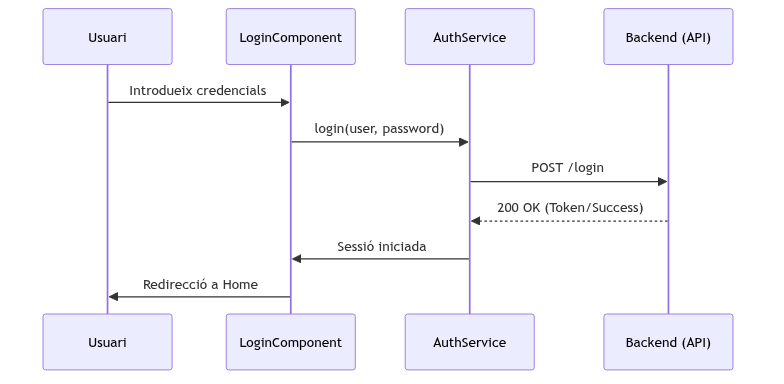
\includegraphics[width=0.85\textwidth]{figures/seq_login.png}
  \caption{Diagrama de seqüència del flux de control d'inici de sessió.}
  \label{fig:seq_login}
  \small Font: Elaboració pròpia.
\end{figure}

\subsection{L'Interceptor de Bloqueig i el Control de Concurrència}
Cal destacar que l'aplicació Angular implementa l'interceptor funcional d'Angular 19 \texttt{authInterceptor} (vegeu el llistat \ref{lst:auth_interceptor_code}). Tanmateix, a diferència de les aplicacions web convencionals on l'interceptor afegeix un token d'usuari, a \textit{Web Core View} aquest s'encarrega d'injectar de forma dinàmica el token de bloqueig d'escriptura (\textbf{Config Lock Token}) adquirit des del servei \texttt{ConfigLockService}. Això assegura que les peticions modificatives cap a les APIs de configuració (\texttt{config.video.*}, \texttt{config.io.*}) estiguin autoritzades per l'exclusivitat del cadenat.

\begin{lstlisting}[language=JavaScript, label={lst:auth_interceptor_code}, caption={Implementació del HttpInterceptorFn per al control del Config Lock en Angular 19.}]
export const authInterceptor: HttpInterceptorFn = (req, next) => {
  const lockService = inject(ConfigLockService);
  const token = lockService.lockToken();
  const isConfigApi = req.url.includes('/config.') || req.url.includes('/resources');
  const isLockOrUnlock = req.url.includes('/properties/lock') || req.url.includes('/properties/unlock');

  if (token && isConfigApi && !isLockOrUnlock) {
    const modifiedReq = req.clone({
      setParams: { token: token }
    });
    return next(modifiedReq);
  }
  return next(req);
};
\end{lstlisting}

\subsection{Subscripció Asíncrona de Temps Real i Notificacions}
Immediatament després d'un inici de sessió reeixit i la redirecció de l'operador cap a la pàgina d'inici de l'aplicació (\texttt{/home}), s'inicialitza la comunicació bidireccional amb el microservei unificat de notificacions. L'aplicació obre un únic canal persistent via WebSocket Segur (\textbf{WSS}) cap al camí \texttt{/ws/la-core-notifier/}.

Aquesta connexió asíncrona unificada és fonamental per rebre d'una sola vegada totes les notificacions de canvis d'estats dels sensors digitals d'E/S, errors globals del maquinari i alertes de pèrdues de senyal de vídeo, evitant que diferents components de la interfície facin peticions redundants o mantinguin múltiples túnels oberts (la qual cosa saturaria la capacitat del gravador).

\subsection{Mecanisme de Keep-Alive i Heartbeat de Sessió}
El manteniment de la sessió es coordina entre el client i el microservei \textbf{la-core-legacy} a través de la persistència del \textit{Heartbeat} emès pel servei \texttt{KeepAliveService}. Aquest mètode executa una crida POST cap al mètode \texttt{KeepAliveSession} de forma periòdica cada 60 segons:

\begin{lstlisting}[language=json, caption={Trama de Keep-Alive enviada periòdicament al servidor.}]
{
  "call": "KeepAliveSession"
}
\end{lstlisting}

\section{Tauler Principal i Panells d'Informació}
La pàgina d'inici (\textit{Home page}) actua com el nucli d'operacions i el despatxador logístic de la plataforma. És la primera interfície que l'operador visualitza un cop el sistema valida correctament les seves credencials en el flux d'autenticació (Figura \ref{fig:ui_home}).

\begin{figure}[htbp]
  \centering
  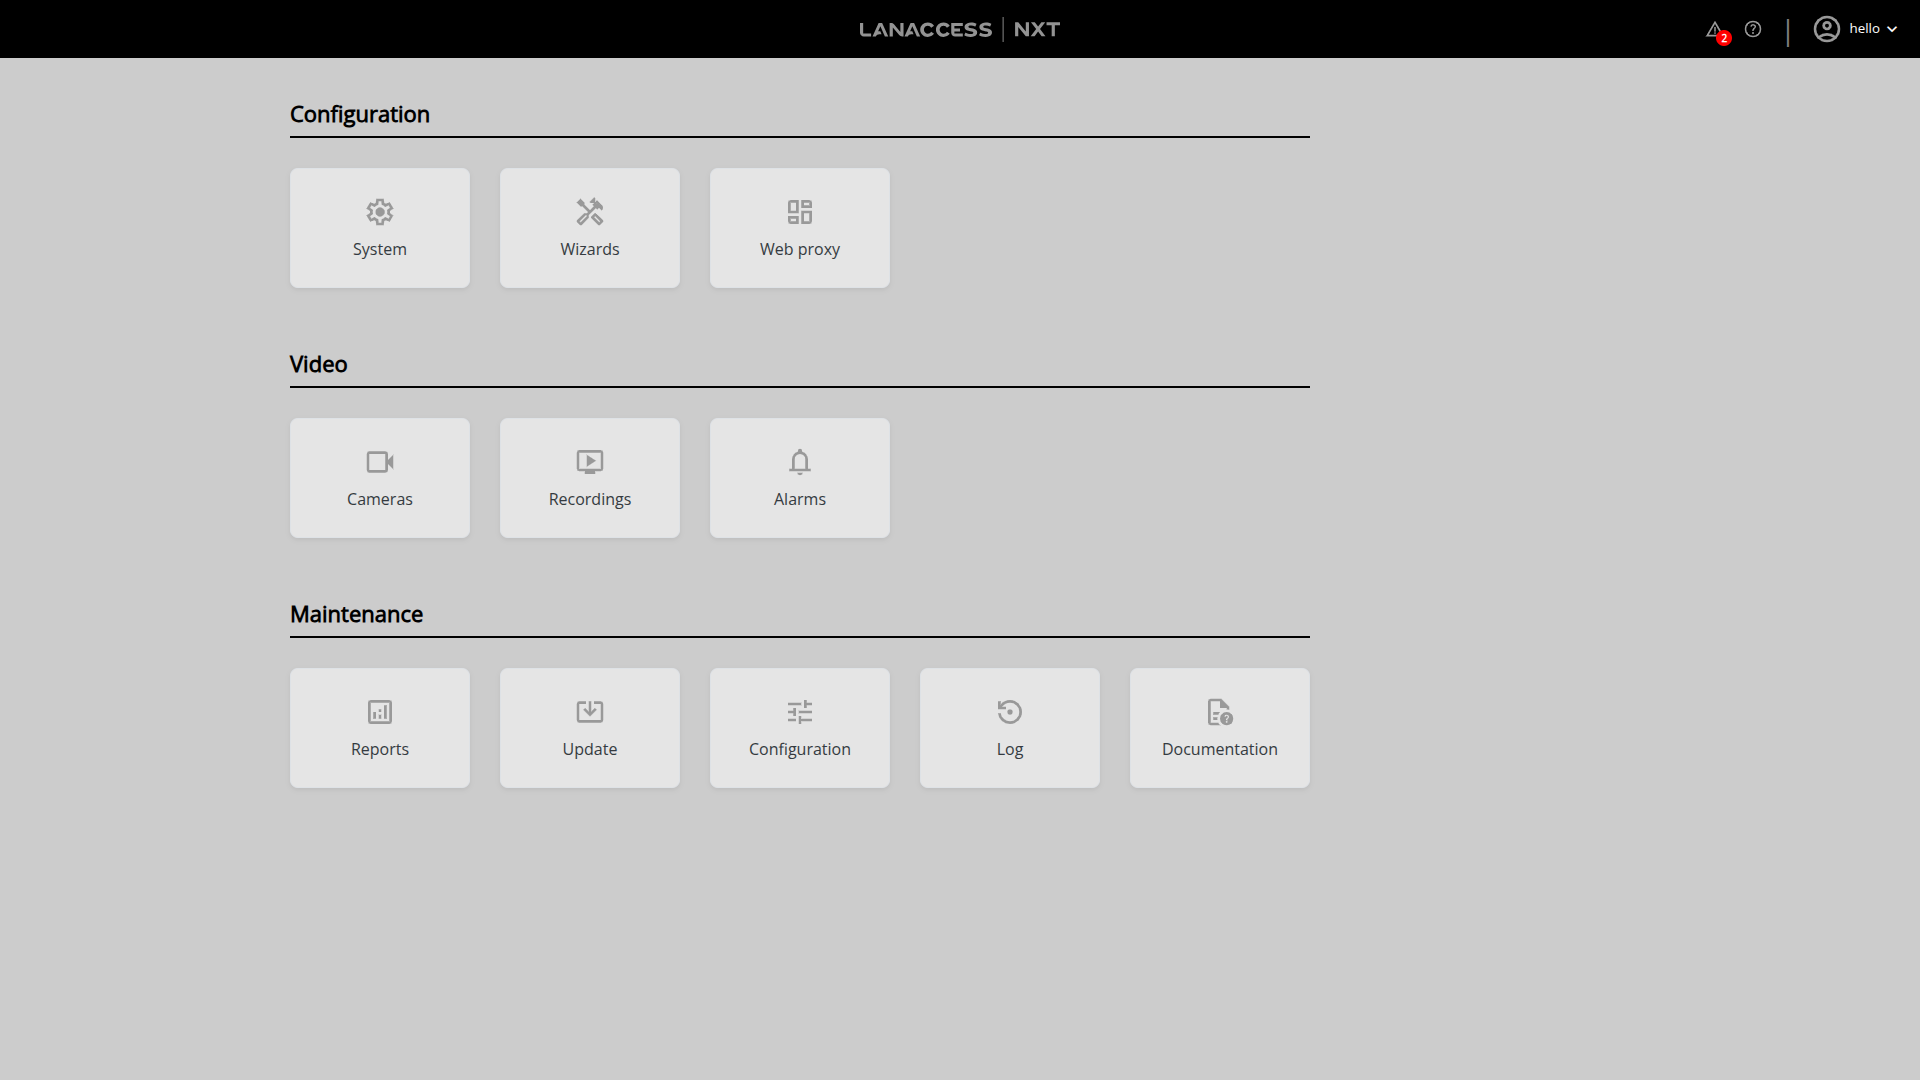
\includegraphics[width=0.95\textwidth]{figures/ui_home.png}
  \caption{Pàgina d'inici principal de Web Core View.}
  \label{fig:ui_home}
\end{figure}

Des d'aquesta pantalla centralitzada, l'usuari pot navegar de manera asíncrona mitjançant el menú de mosaic o utilitzar els controls globals de la capçalera de l'aplicació per accedir a les diferents eines operatives.

\subsection{Organització de Funcionalitats i Autorització Dinàmica}
Per garantir una experiència d'usuari (UX) neta, adaptada al context de treball i lliure de sobrecàrregues cognitives, les eines del sistema s'organitzen visualment en tres grans seccions funcionals:

\begin{itemize}
  \item \textbf{Configuració:} Reuneix l'accés a la configuració del sistema (\textit{System}), els assistents guiats d'instal·lació (\textit{Wizards}) i l'eina de mapeig de túnels de xarxa per a càmeres aïllades (\textit{Web Proxy}).
  \item \textbf{Vídeo:} Agrupa el visualitzador de càmeres en temps real (\textit{Cameras}), la consulta del reproductor històric de gravacions (\textit{Recordings}) i la consola de supervisió d'incidents actius (\textit{Alarms}).
  \item \textbf{Manteniment:} Conté els mòduls de diagnòstic avançat (\textit{Reports}), actualització del microprogramari (\textit{Update}), restauració i còpies de seguretat de fitxers de configuració (\textit{Configuration}), el visor de registres històrics (\textit{Log}) i la descàrrega directa de manuals d'usuari integrats (\textit{Documentation}).
\end{itemize}

L'aspecte més destacable d'aquest disseny és que el motor de renderitzat del *frontend* avalua de forma immediata el mètode reactiu \texttt{functionalities} derivat de la llista de \textit{grants} de l'usuari a través d'Angular Signals. Si l'operador actual manca d'un permís determinat (com ara l'accés a la modificació d'usuaris o a l'actualització de firmware), els botons i rutes d'aquella secció específica s'exclouen directament del cicle de vida del DOM del client. Això no només augmenta la seguretat en l'entorn de treball, sinó que evita la renderització d'elements redundants que l'usuari final no pot utilitzar.

\subsection{Controls Globals i Panells d'Informació de Maquinari i Usuari}
A la part superior dreta de l'aplicació, dins de la barra de capçalera persistent, s'ubiquen els controls d'accés ràpid i els panells flotants en temps real (Figura \ref{fig:ui_home_panels}).

\begin{figure}[htbp]
  \centering
  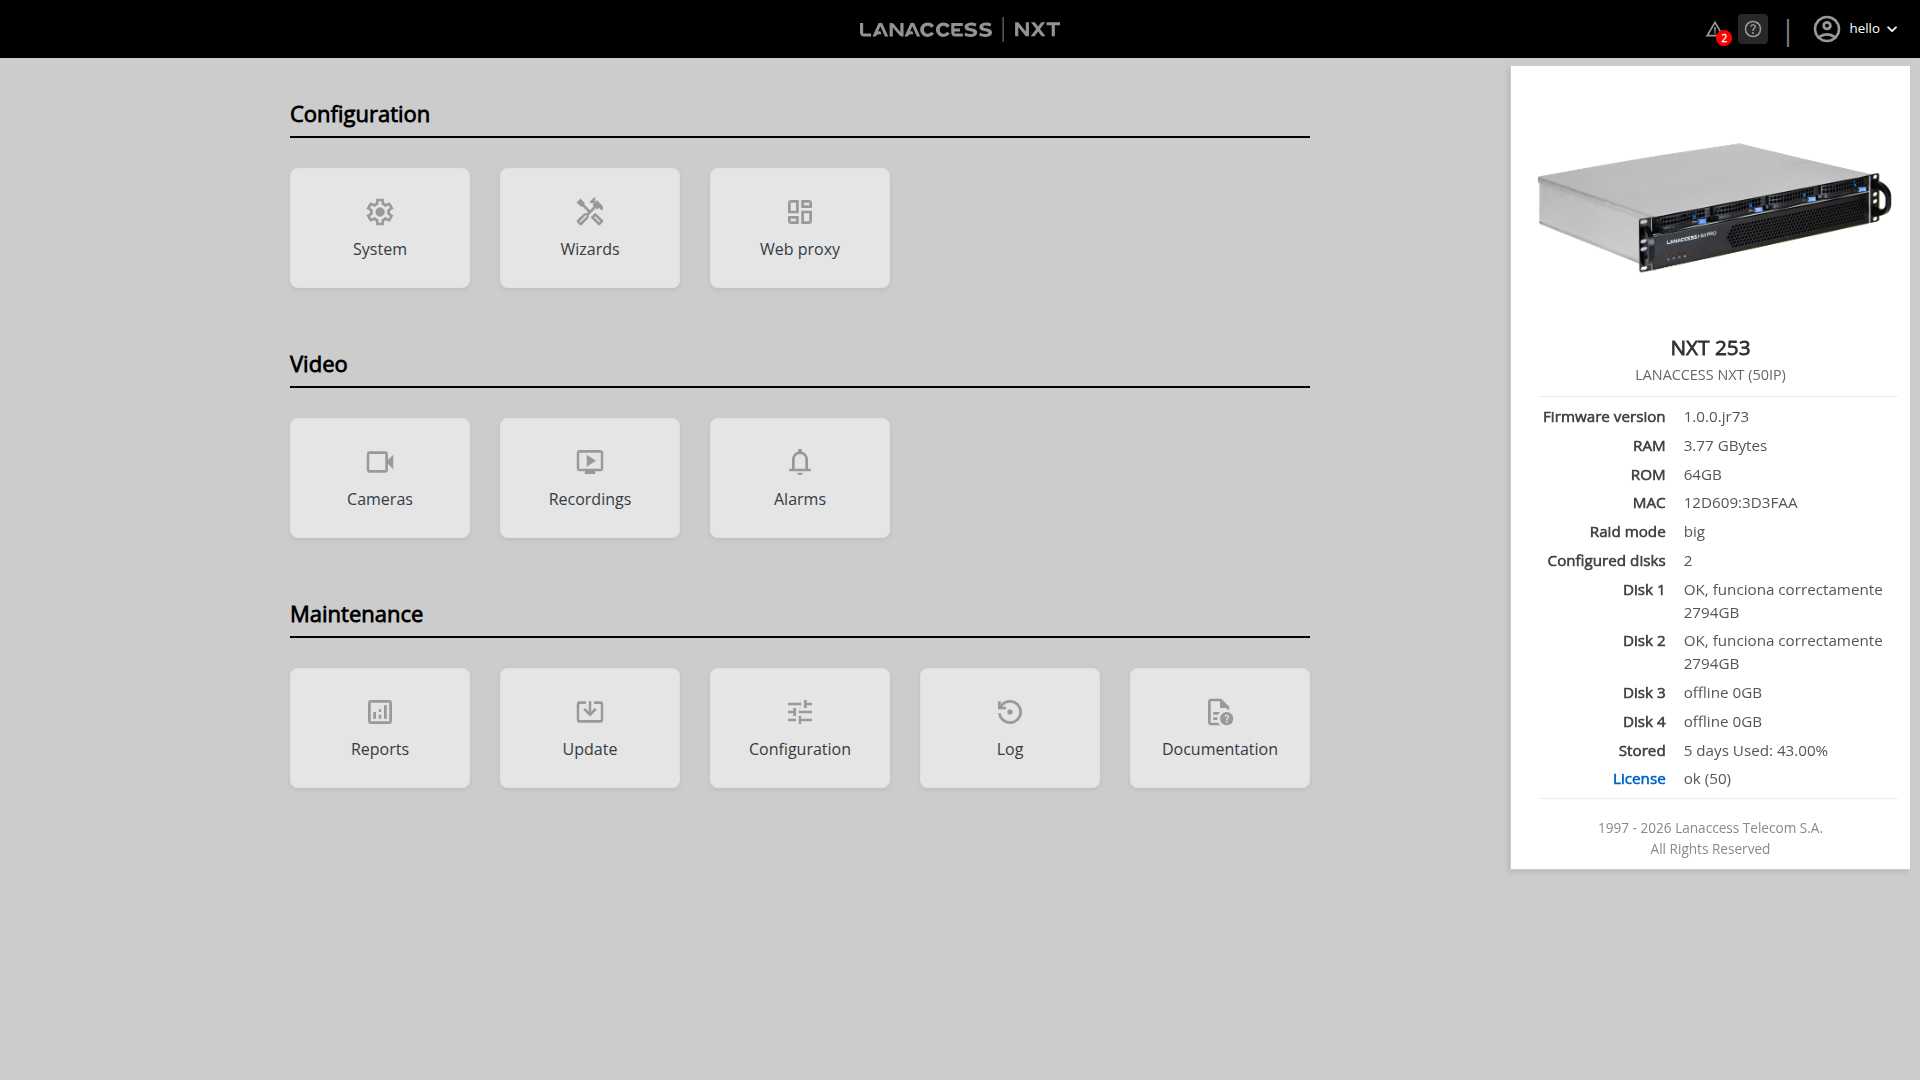
\includegraphics[width=0.45\textwidth]{figures/ui_home_info.png}
  \hfill
  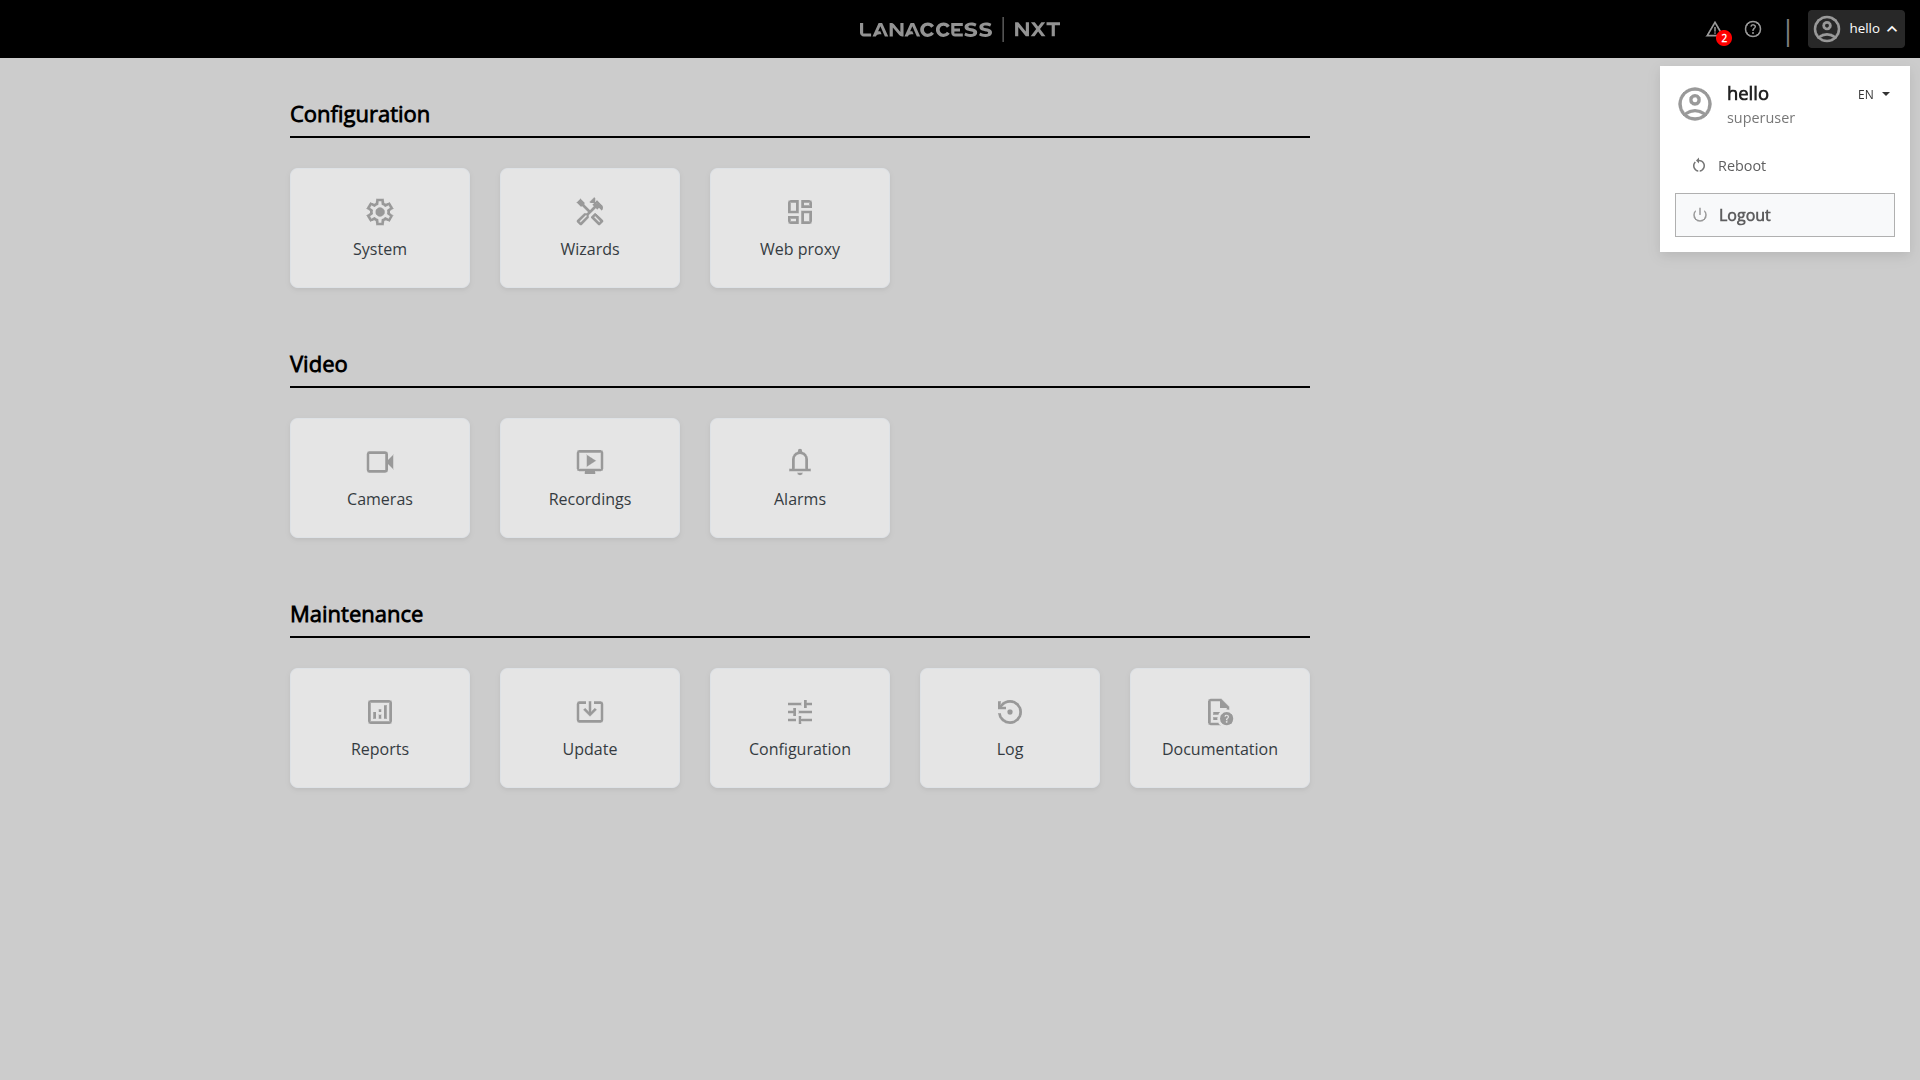
\includegraphics[width=0.45\textwidth]{figures/ui_home_user.png}
  \caption{Panell d'informació de l'estat del videogravador (esquerra) i d'usuari (dreta).}
  \label{fig:ui_home_panels}
\end{figure}

Fent clic a la icona d'informació de maquinari, es desplega un panell lateral que actua com a diagnòstic ràpid de l'estat de salut de l'NVR (Figura \ref{fig:ui_home_panels}, esquerra). Aquest panell mostra paràmetres crítics obtinguts directament del maquinari de forma asíncrona:
\begin{itemize}
  \item Adreça IP local i adreça física MAC de la interfície \texttt{eth0}.
  \item Versió del firmware del sistema operatiu i model del dispositiu de gravació.
  \item \textbf{Estat de l'emmagatzematge físic:} Llista normalitzada dels discos durs muntats al sistema, detallant-ne la capacitat, el model de fabricant, el número de sèrie, el mode de redundància de dades (RAID) actiu i el percentatge d'espai utilitzat.
  \item Temperatura del processador central obtinguda directament dels sensors integrats.
  \item \textbf{Estat de la llicència:} Des d'aquest panell d'informació del videogravador podem veure l'estat actual de la llicència, amb un botó accionable que redirigeix directament a la pàgina de llicència.
\end{itemize}

Per alimentar aquest panell de diagnòstic, el frontend realitza una petició HTTP GET cap a la ruta d'API xifrada \texttt{/webprotocol/config\_data.xml?requests=system+network}. El microservei \textbf{la-core-legacy} s'encarrega d'analitzar les variables del sistema, unificar les metadades en un fitxer estructurat XML i transmetre'l cap a l'aplicació web, la qual l'interpreta asíncronament sense necessitat de recarregar la pàgina.

Al seu costat, el panell d'usuari (Figura \ref{fig:ui_home_panels}, dreta) detalla el nom de l'operador actiu i el perfil assignat pel sistema, complint amb el requisit d'autenticació basat en rols (RF-1.1). Aquest panell unifica tres accions globals clau per al funcionament de l'equip:
\begin{enumerate}
  \item \textbf{Tancament de sessió segur:} Un botó d'apagat físic que realitza una petició POST cap a l'endpoint \texttt{/WebLogin} amb l'acció \texttt{Logout}. Aquesta operació destrueix les credencials del servidor de manera immediata i buida completament el Signal privat de la memòria de l'aplicació web per evitar que la sessió quedi accessible.
  \item \textbf{Reinici remot del gravador:} Un botó que executa la comanda de reinici físic del videogravador coordinada pel servei \texttt{MaintenanceService}. Aquesta acció obre un flux de comunicació securitzat amb el backend i mostra un component d'espera que supervisa el procés de reinici físic del maquinari.
  \item \textbf{Selector d'idioma d'interfície:} Un desplegable reactiu que permet commutar de manera immediata l'idioma de l'aplicació web entre l'anglès, l'espanyol i el francès. Aquesta funcionalitat es gestiona mitjançant el mecanisme d'internacionalització (\textit{i18n}) d'Angular gràcies a la llibreria \texttt{ngx-translate}. Els fitxers de traducció JSON es carreguen de forma dinàmica i s'actualitzen en el DOM sense requerir la recàrrega del navegador.
\end{enumerate}

\subsection{Gestió de Llicències}
Accedint a través del botó del panell d'informació, l'operador és redirigit a la pàgina de llicència (Figura \ref{fig:ui_license}). En aquesta pantalla es mostra el resum de l'estat legal i operatiu del sistema, on s'especifica informació clau com el nombre màxim de canals de vídeo permesos per la llicència actual, i permet procedir a l'activació o renovació de la mateixa quan sigui necessari.

\begin{figure}[htbp]
  \centering
  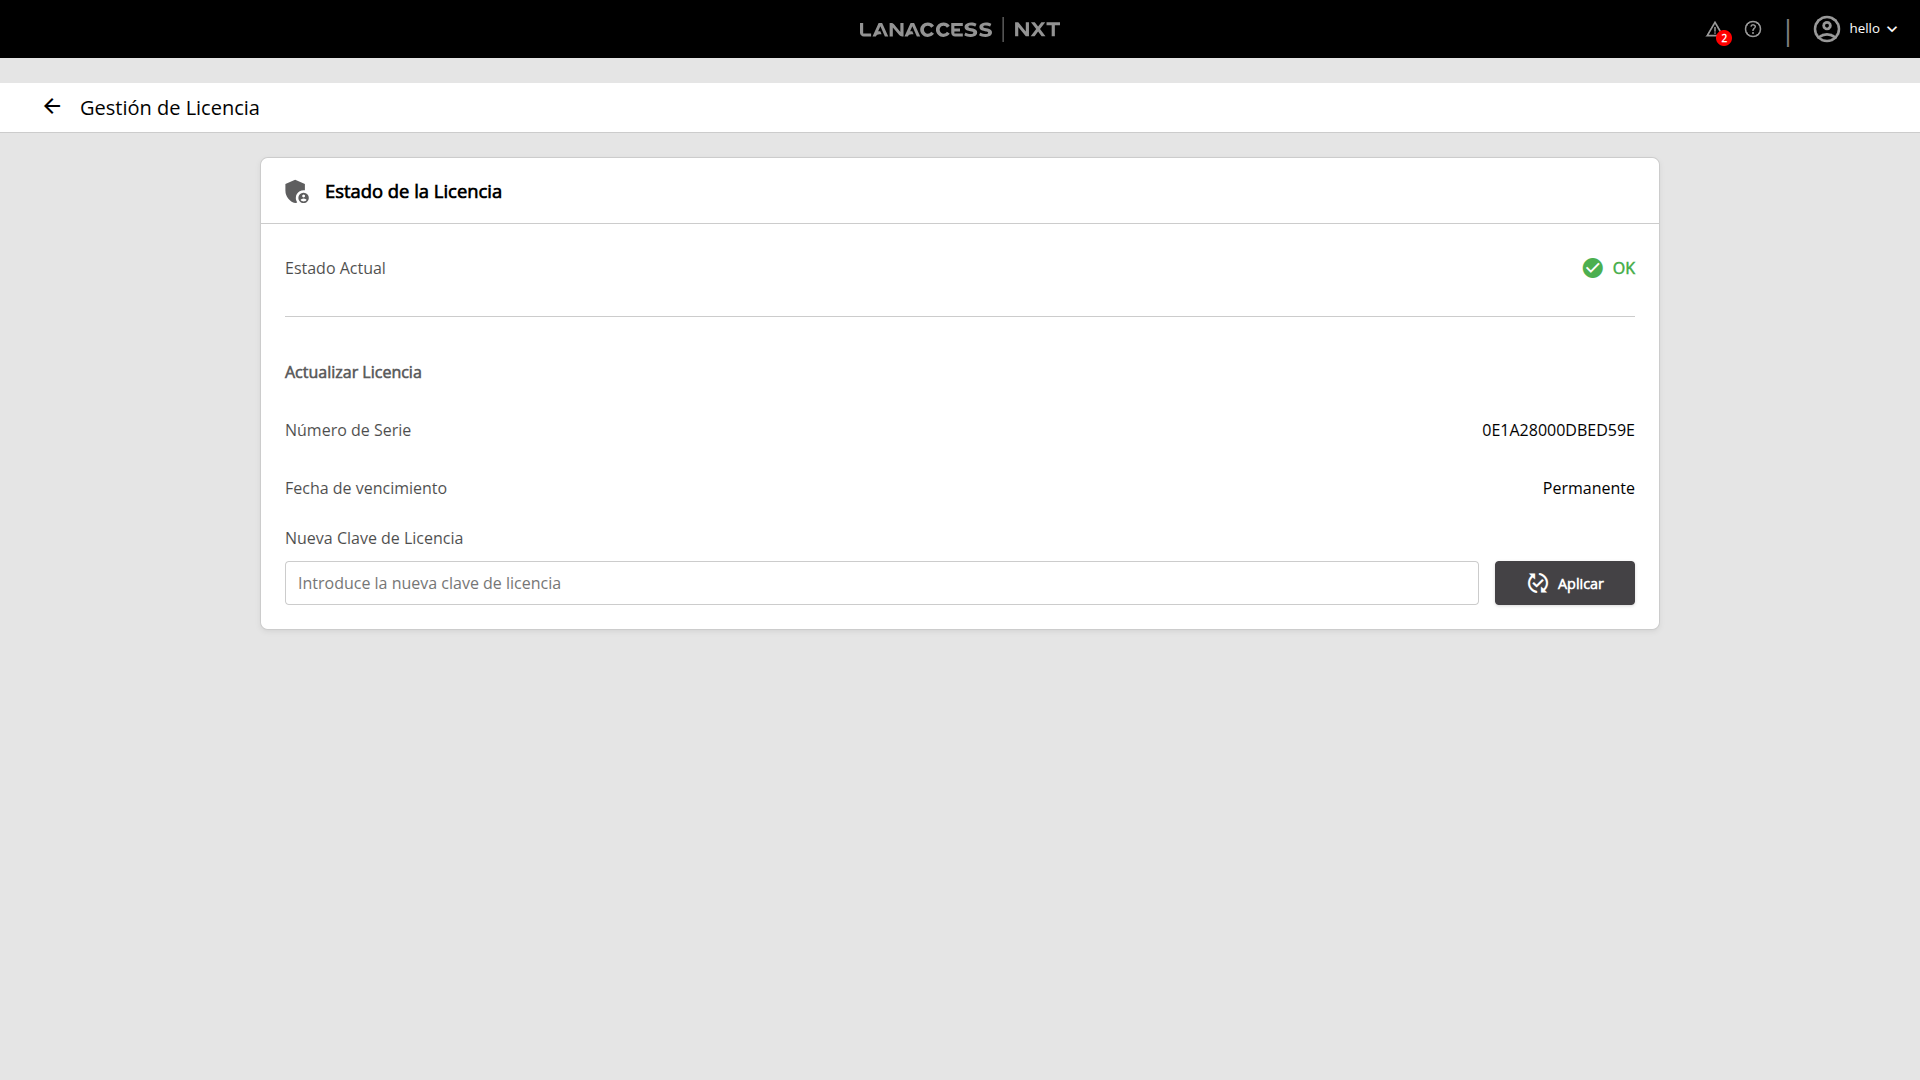
\includegraphics[width=0.95\textwidth]{figures/ui_license.png}
  \caption{Pàgina de gestió de la llicència del sistema.}
  \label{fig:ui_license}
\end{figure}

\subsection{Sistema unificat d'alertes en temps real i canal de notificacions}
Un element clau de la capçalera és la icona de la campana de notificacions (Figura \ref{fig:ui_errors}). La seguretat industrial exigeix que qualsevol anomalia física o lògica (com la pèrdua de senyal d'una càmera, una fallida en un disc d'emmagatzematge o un atac contra el sistema de xarxa) es comuniqui a l'instant.

\begin{figure}[htbp]
  \centering
  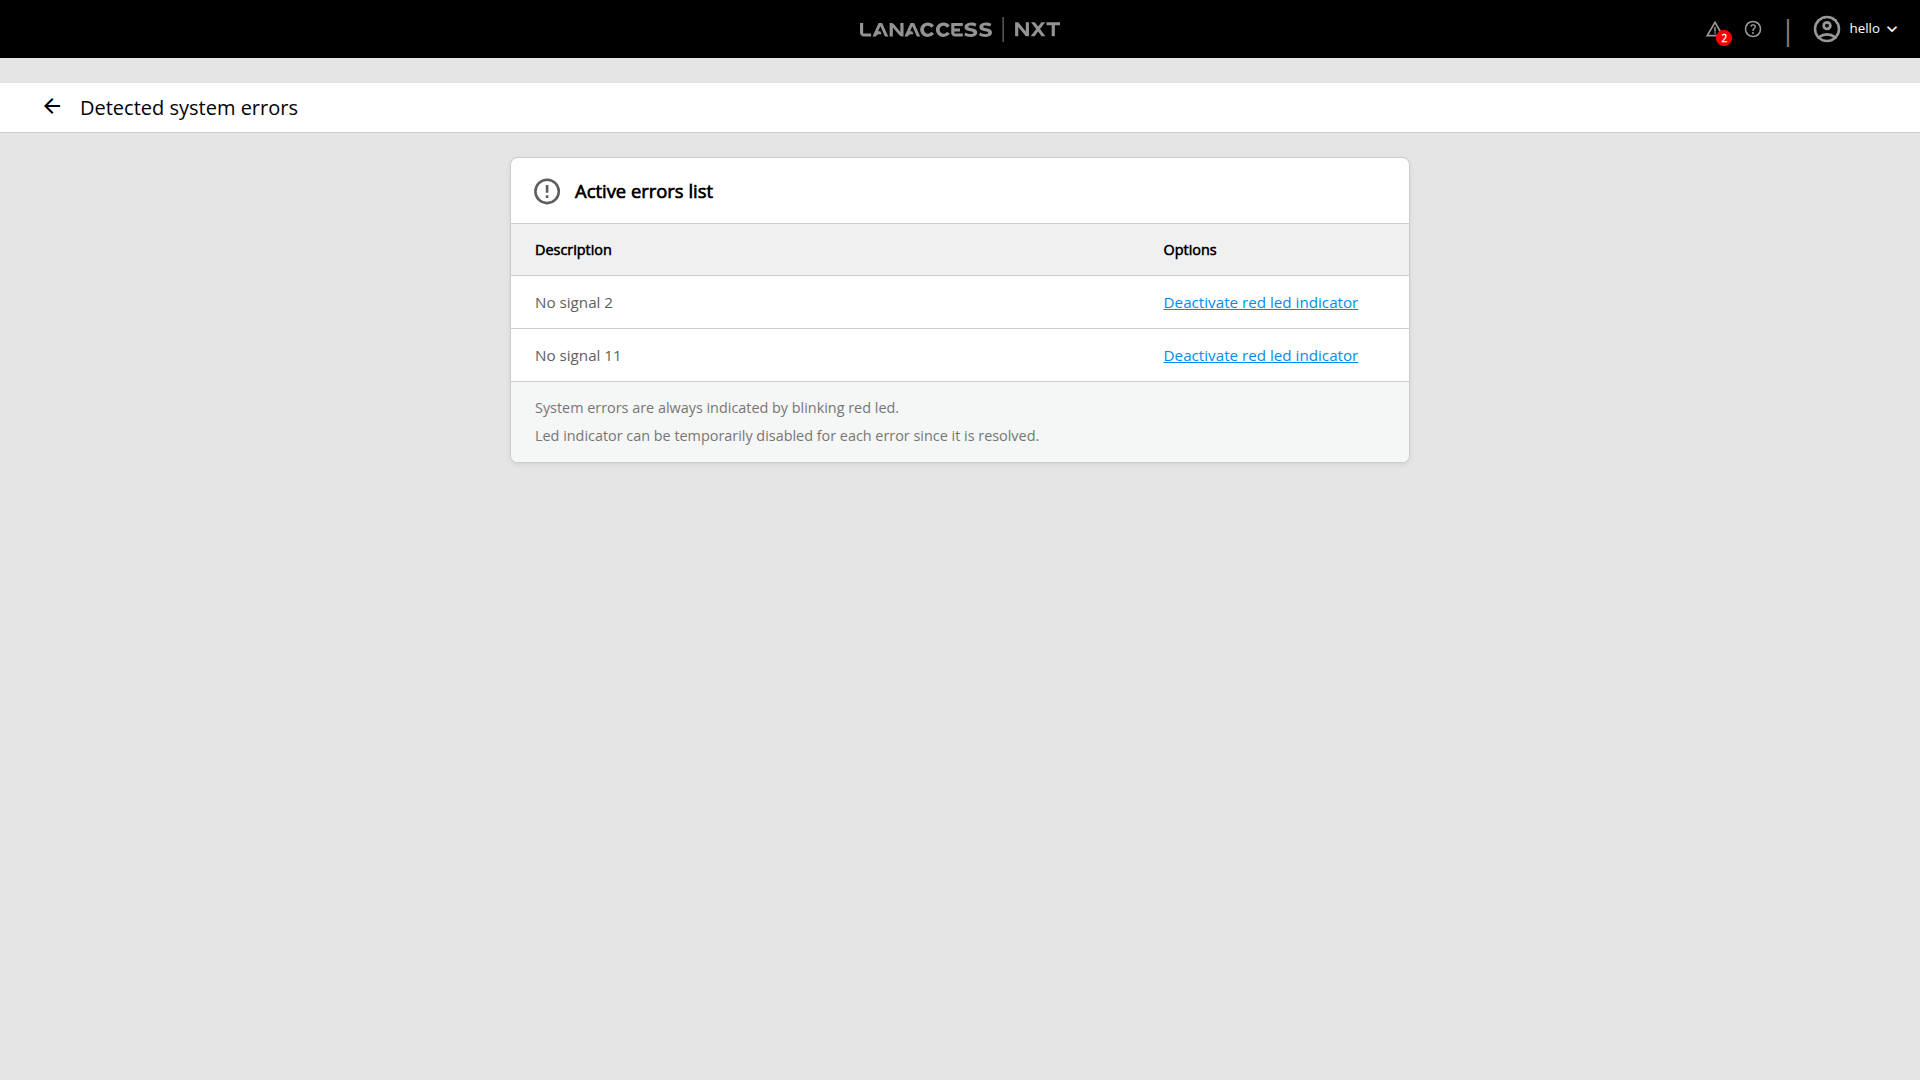
\includegraphics[width=0.95\textwidth]{figures/ui_errors.png}
  \caption{Sistema de notificacions i errors emergents.}
  \label{fig:ui_errors}
\end{figure}

Per aconseguir-ho, l'aplicació implementa una subscripció asíncrona persistent mitjançant el servei de notificacions d'errors unificat (\texttt{AlertService}). Aquest servei manté una connexió constant via WebSocket Segur amb el microservei \textbf{la-core-notifier}. Quan es produeix un esdeveniment a l'NVR, aquest és publicat al bus intern de Linux \textbf{D-Bus}. El servei de notificacions llegeix el senyal, el converteix en un missatge estructurat amb el format \texttt{ERRORS\_NOTIFY} i el transmet immediatament cap al frontend per fer aparèixer un globus de notificació (\textit{badge}) amb el nombre d'alertes pendents sobre la icona de la campana.

Si l'operador fa clic sobre aquest indicador, el sistema el redirigeix cap al panell de diagnòstic d'errors actius (Figura \ref{fig:ui_errors}), on es mostren en detall les fallides actives del sistema, podent interaccionar directament per apagar el senyal de led de l'alarma des de la pantalla web un cop s'ha revisat la incidència.

\section{Configuració del Sistema i Motor Dinàmic (Schema-Driven)}
El disseny de la gestió de configuració de la plataforma \textit{Web Core View} representa una evolució significativa respecte als mètodes tradicionals basats en formularis estàtics o fitxers de configuració dispersos. En lloc de duplicar la lògica de validació al front-end, s'ha implementat una arquitectura de \textbf{Soberania del Backend} (\textit{Backend-Driven Development}), on el gravador NXT actua com a única font de veritat (\textit{Single Source of Truth}).

Dins de l'abast d'aquest projecte, s'ha dissenyat conjuntament amb l'equip d'embedded l'estructura de comunicació de dades i els mecanismes d'hidratació, i s'ha implementat completament en el costat del client el motor d'interpretació dinàmica capaç de transformar metadades JSON en interfícies d'usuari interactives, validades i robustes de manera autònoma.

\subsection{El Model de Validació en Cascada (Cascaded Validation)}
Per evitar l'anomenada \textit{"Configuració Fantasma"} (per exemple, que l'usuari pugui programar gravacions d'una càmera o d'un sensor físicament inexistent), el sistema organitza la informació en un model de validació estructural de tres capes que es complementen de forma jeràrquica:

\begin{enumerate}
  \item \textbf{Capa Teòrica (Esquema):} Defineix les regles abstractes de joc i els límits teòrics del programari de manera declarativa mitjançant fitxers YAML integrats al servei de validació de l'NVR (ex: \textit{"el sistema admet un màxim de 32 entrades"}).
  \item \textbf{Capa Física (Recursos - \texttt{/resources}):} Exposa el maquinari realment connectat o llicenciat en l'equip en temps d'execució mitjançant un conjunt d'APIs REST complementàries (ex: \textit{"aquest equip disposa d'un mòdul físic amb 8 entrades instal·lades"}).
  \item \textbf{Capa Lògica (Dades de Configuració):} Representa l'arbre de configuració real que l'operador decideix aplicar (ex: \textit{"activa la gravació quan l'entrada 3 estigui activa"}).
\end{enumerate}

\begin{figure}[htbp]
  \centering
  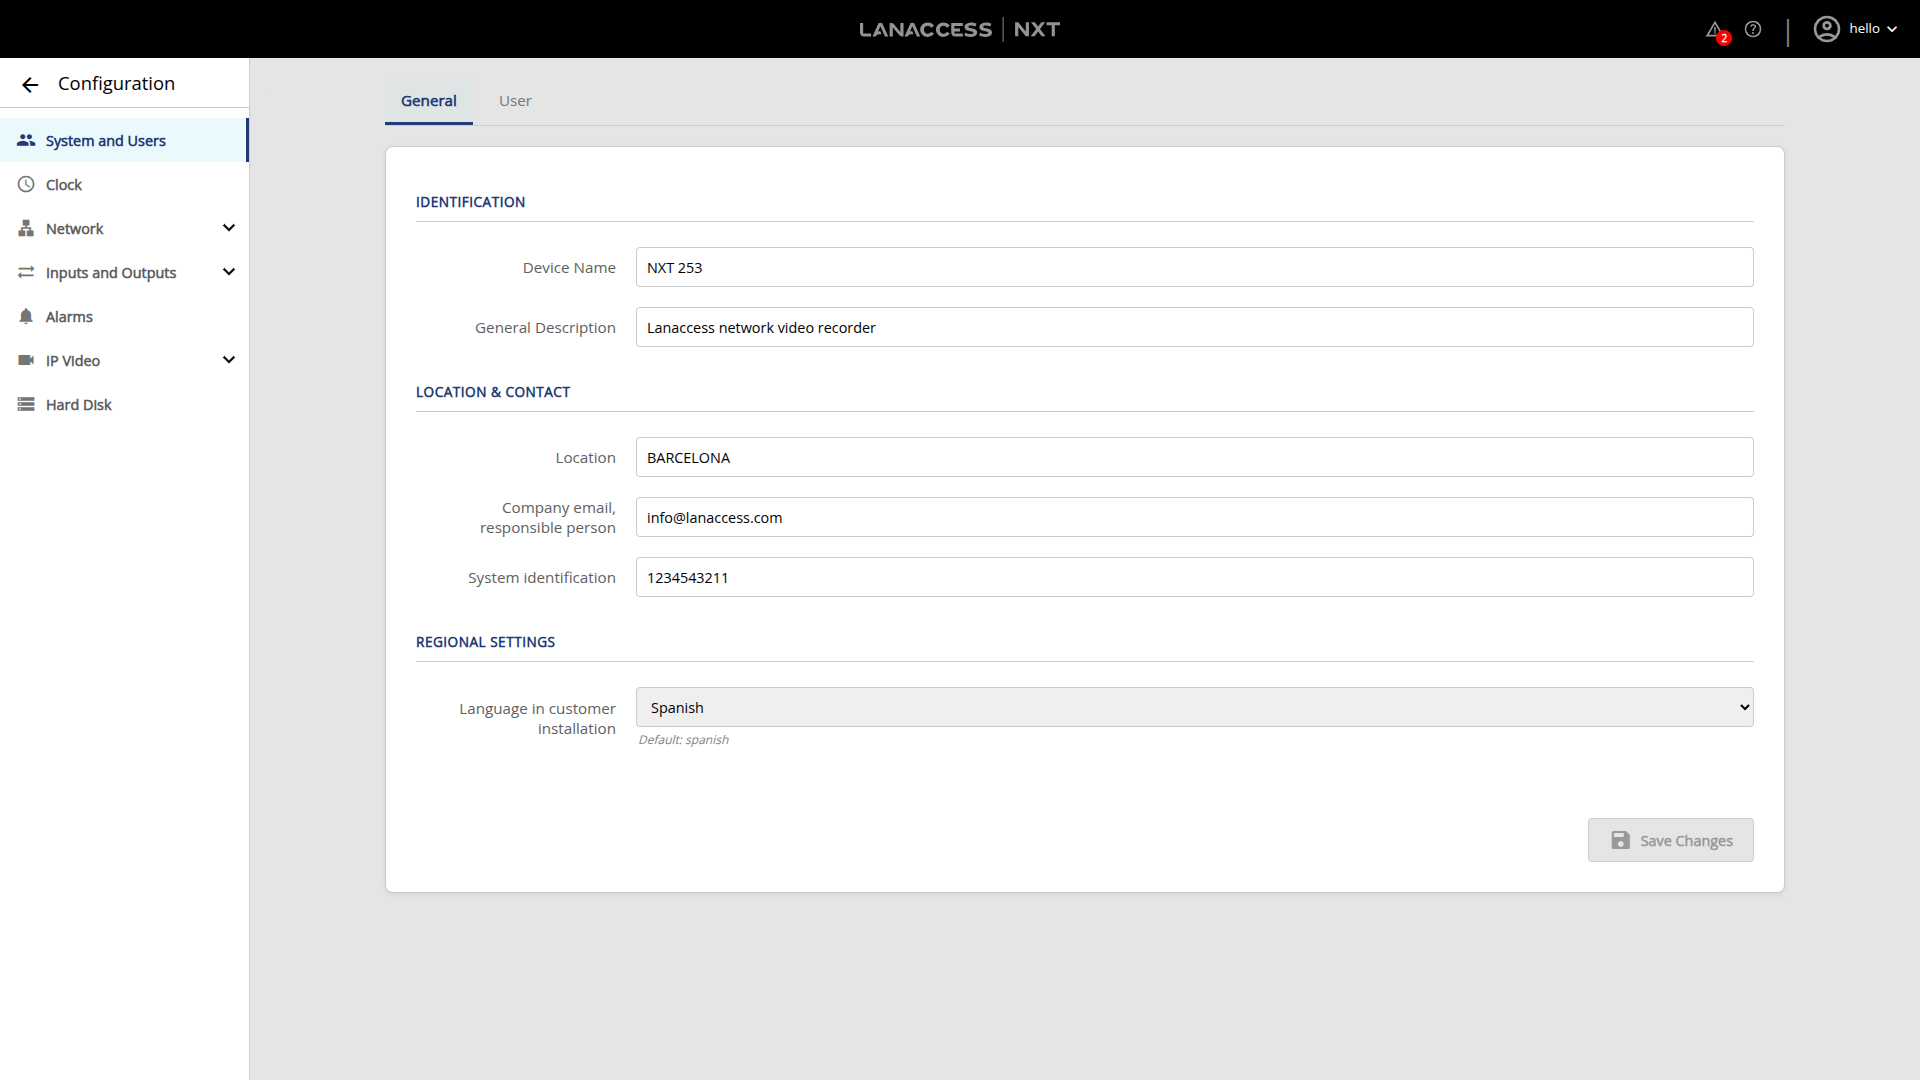
\includegraphics[width=0.95\textwidth]{figures/ui_system1.png}
  \caption{Pantalla de configuració principal del sistema generada dinàmicament.}
  \label{fig:ui_system1}
\end{figure}

Mitjançant aquesta validació en cascada, el client d'Angular consulta de manera proactiva la capa de recursos i l'esquema de dades abans de dibuixar l'interfície. Si l'operador intenta forçar una petició d'escriptura invàlida, el servidor la rebutja immediatament amb un error \texttt{HTTP 422 Unprocessable Entity}.

\subsection{Projecció Virtual i Hidratació de Dades (Merge Logic)}
Internament, per garantir un temps d'accés $O(1)$ i l'eficiència en sistemes de memòria flaix limitats, l'NVR emmagatzema les dades de configuració en un format pla de tipus clau-valor a través del bus del sistema (\texttt{D-Bus}). Tanmateix, per a l'API REST de cara al frontend, el servei \texttt{la-core-legacy} fa una projecció d'aquestes claus per reconstruir en temps real un arbre de dades jeràrquic i tipat en format JSON (Figura \ref{fig:ui_system2}).

\begin{figure}[htbp]
  \centering
  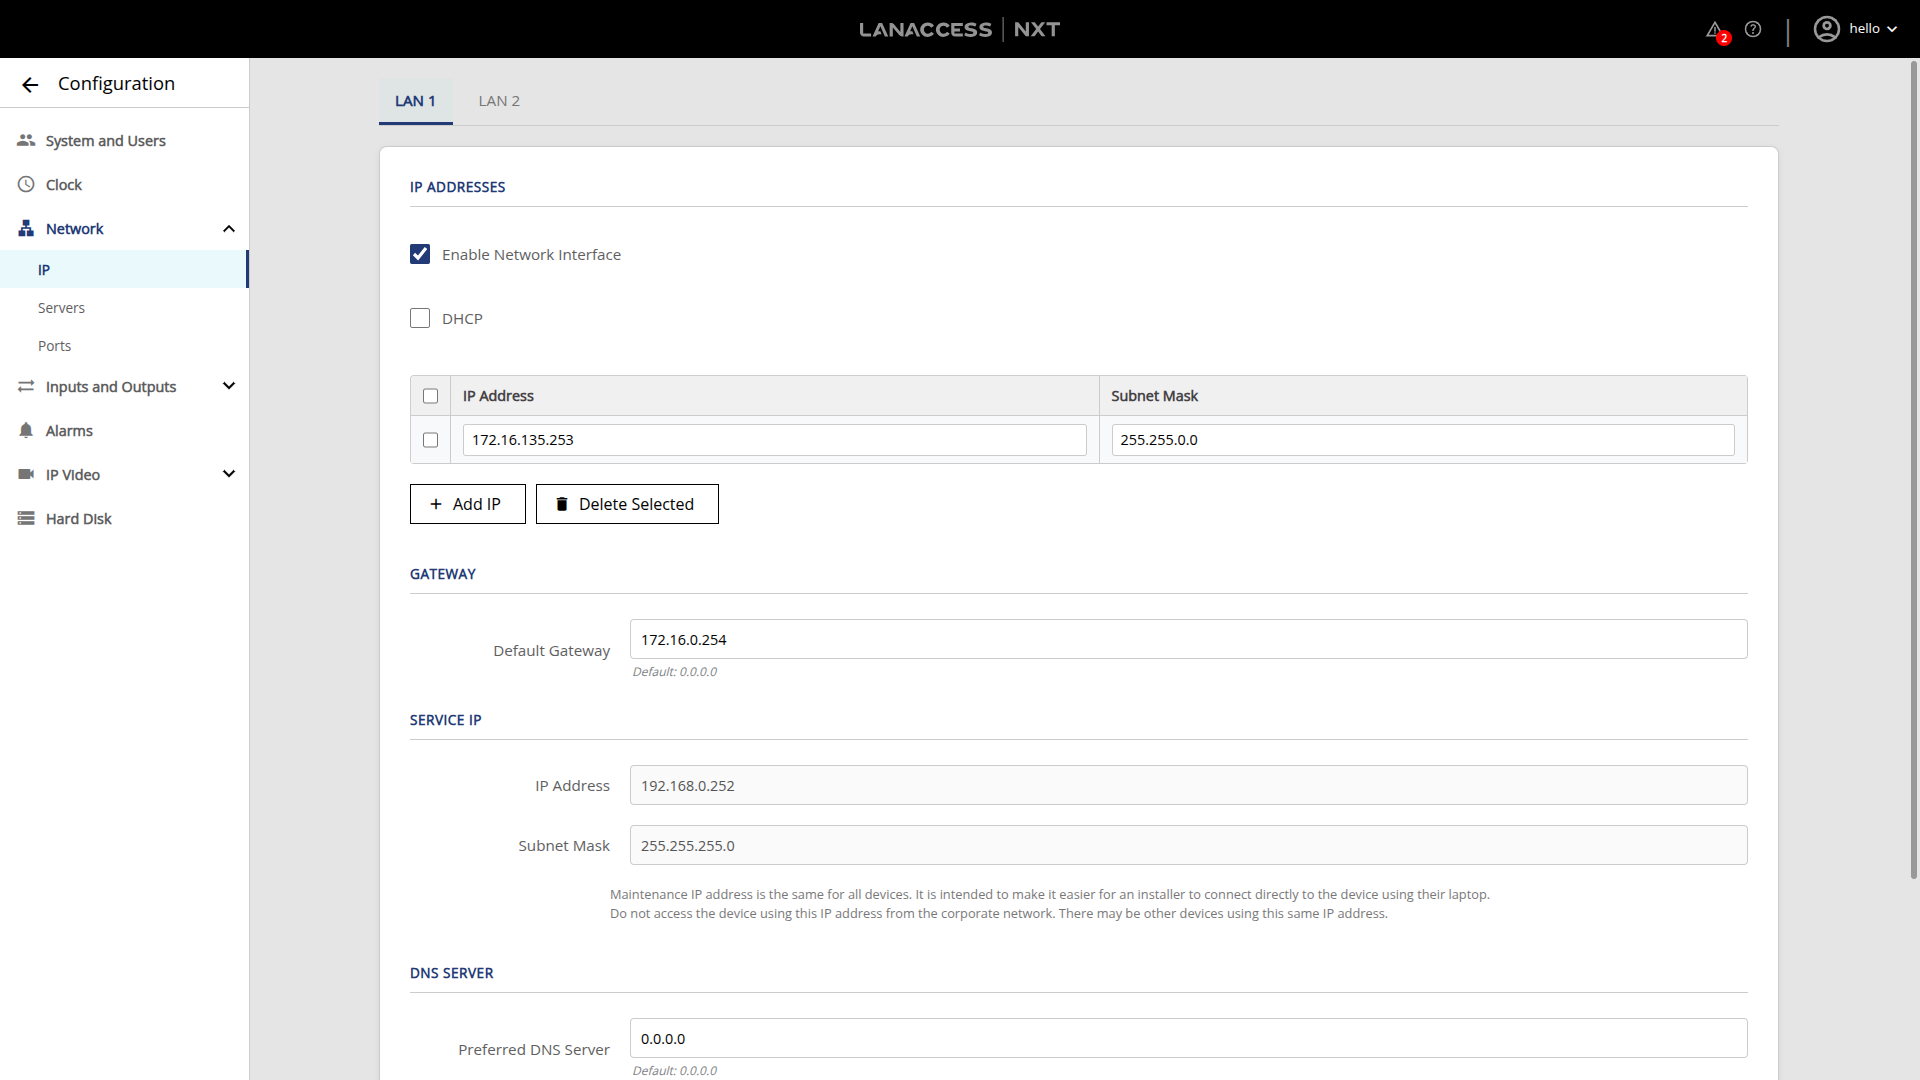
\includegraphics[width=0.95\textwidth]{figures/ui_system2.png}
  \caption{Detall de l'edició de paràmetres de xarxa i interfícies.}
  \label{fig:ui_system2}
\end{figure}

Durant les operacions de lectura (\texttt{GET}), l'API del servidor realitza una operació d'hidratació de dades (\textit{Merge}):
\begin{enumerate}
  \item Carrega de la persistència les dades modificades per l'usuari.
  \item Recorre l'esquema del node en paral·lel. Per a cada propietat que no estigui definida en la persistència, hi injecta automàticament el seu valor per defecte (\texttt{\_default}).
  \item Genera de manera automàtica totes les instàncies lògiques per a col·leccions fixes definides pel maquinari (ex: cam01 a cam16), evitant que l'aplicació Angular hagi d'omplir buits amb lògica condicional defensiva.
\end{enumerate}

\subsection{Motor Dinàmic del Frontend (Schema-Driven Rendering)}
El client web actua com un intèrpret asíncron de les definicions d'esquema exposades per l'endpoint \texttt{/device-service/properties/schema}. El component dinàmic \texttt{ConfigInputComponent} rep la definició i renderitza de forma autònoma el component de presentació equivalent, utilitzant un flux recursiu basat en el tipus semàntic de la propietat d'esquema, tal com s'il·lustra a la Figura \ref{fig:ui_system3}:

\begin{itemize}
  \item \texttt{\_type: "boolean"}: Es renderitza mitjançant un commutador (\texttt{ToggleComponent}).
  \item \texttt{\_type: "integer" / "numeric"}: Si té restriccions de màxims i mínims, genera un element lliscant (\texttt{SliderComponent}) o un camp numèric normalitzat.
  \item \texttt{\_type: "list"}: Genera un selector de llista desitjada (\texttt{SelectComponent}) basat en els elements del vector \texttt{\_allowedValues}.
  \item \texttt{\_type: "flag"}: Configura una màscara de selecció múltiple.
  \item \texttt{\_type: "resource\_list" / "resource\_flag"}: Modifica la llista d'opcions connectant dinàmicament el selector amb les instàncies del maquinari real obtingut prèviament d'una consulta a \texttt{/resources}.
\end{itemize}

\begin{figure}[htbp]
  \centering
  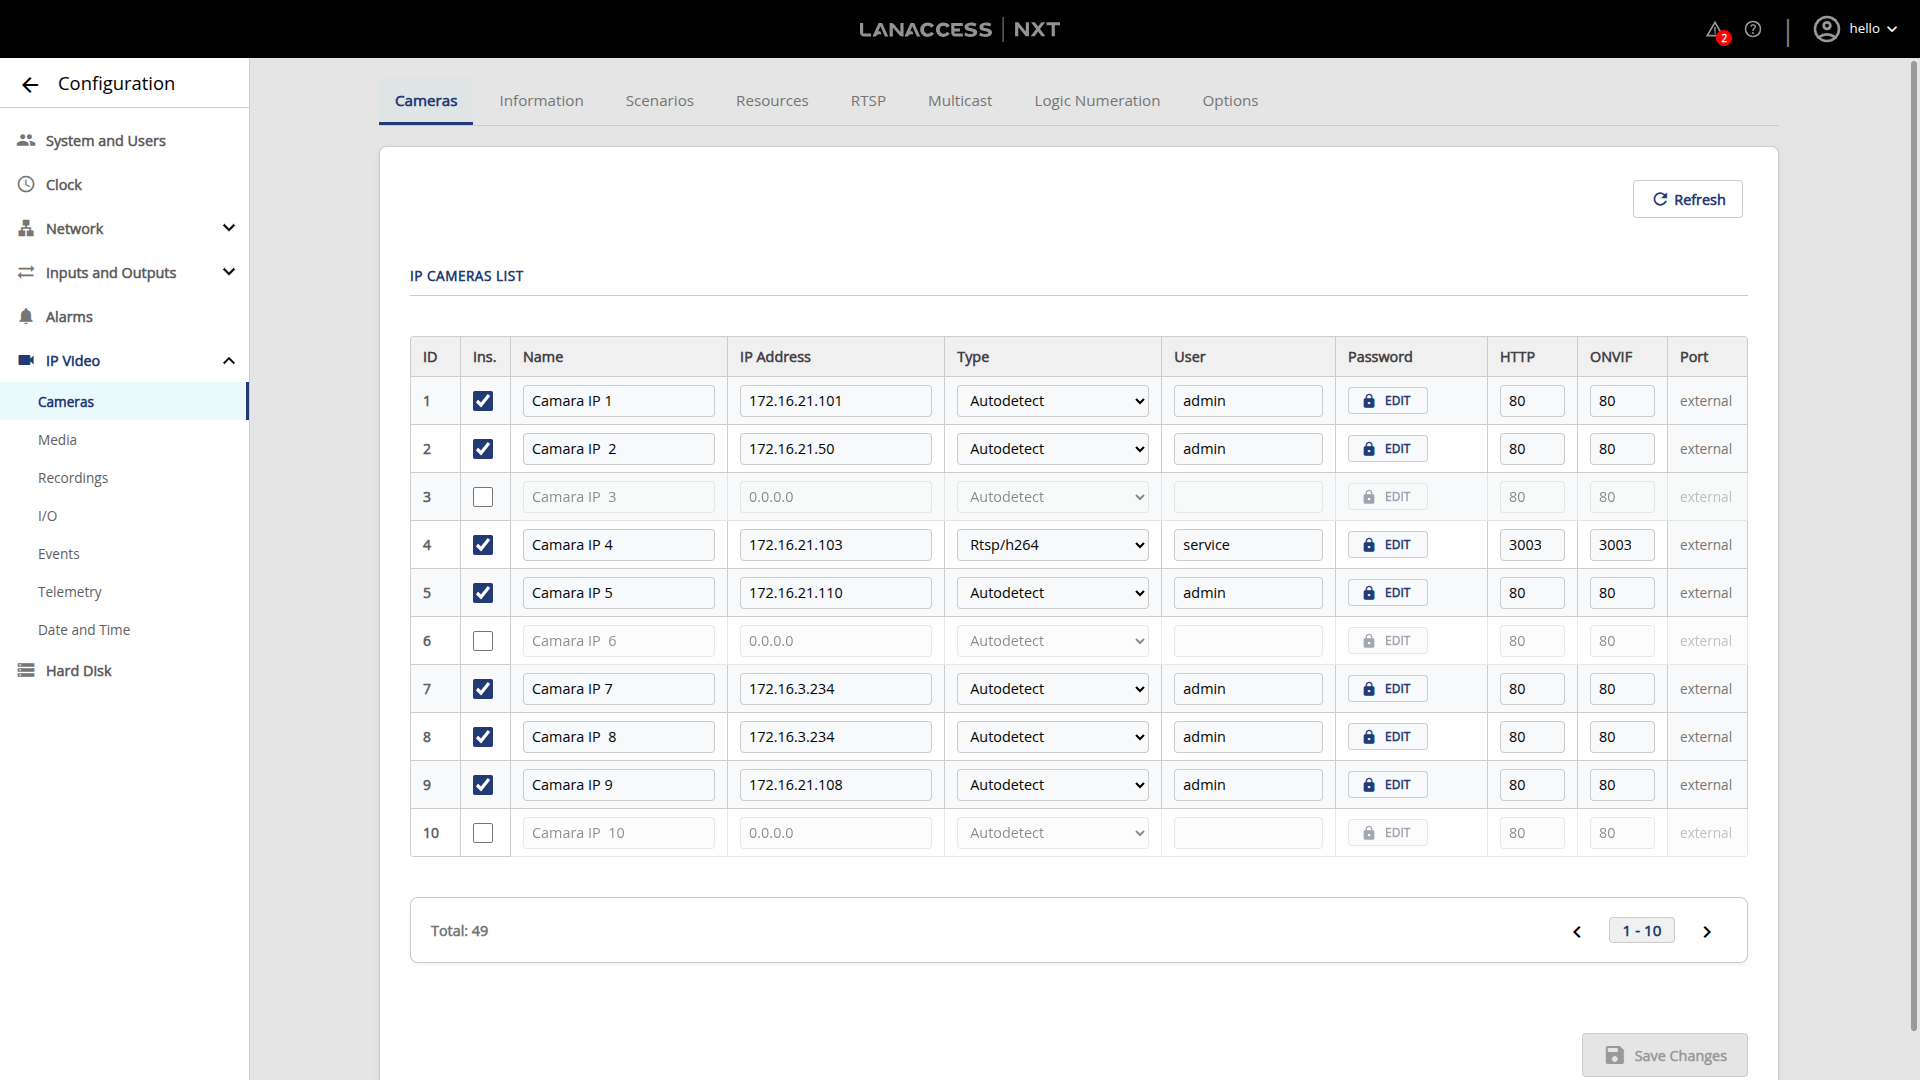
\includegraphics[width=0.95\textwidth]{figures/ui_system3.png}
  \caption{Desplegables (\textit{selects}) i botons commutadors (\textit{toggles}).}
  \label{fig:ui_system3}
\end{figure}

\subsection{Validació Dinàmica de Tipus i Formats amb Signals}
Per garantir la integritat de les dades del costat de client i guiar l'operador abans de fer l'enviament, s'ha programat una variable reactiva calculada (\textit{computed signal}) anomenada \texttt{computedValidationError}. Aquesta avalua de forma instantània el valor escrit contra les regles declaratives de l'esquema:

\begin{lstlisting}[language=JavaScript, caption={Lògica de validació dinàmica amb \textit{Signals} i \textit{Regex} a ConfigInputComponent.}]
computedValidationError = computed(() => {
  const value = this.inputValue();
  const def = this.fieldDef();
  if (!def) return null;

  // 1. Validacio de patrons d'expressio regular (ex: IP, Mascara, Domain)
  if (def._regex) {
    const rx = new RegExp(def._regex);
    if (!rx.test(String(value))) {
      return def._description || 'Format invalid';
    }
  }

  // 2. Validacio de limits numerics de rang
  if (def._type === 'integer' || def._type === 'numeric' || def._type === 'decimal') {
    const minVal = def._min !== undefined ? def._min : def._minValue;
    const maxVal = def._max !== undefined ? def._max : def._maxValue;
    if (minVal !== undefined && value < minVal) return `Minim: ${minVal}`;
    if (maxVal !== undefined && value > maxVal) return `Maxim: ${maxVal}`;
  }

  // 3. Validacio de longituds de text
  if (def._type === 'string') {
    if (def._minLength && String(value).length < def._minLength) {
      return `Minim ${def._minLength} caracters`;
    }
    if (def._maxLength && String(value).length > def._maxLength) {
      return `Maxim ${def._maxLength} caracters`;
    }
  }
  return null;
});
\end{lstlisting}

\subsection{Gestió de Centineles i Valors Buits}
Un repte arquitectònic clau d'aquest model híbrido (dades jeràrquiques sobre disc pla clau-valor) és el tractament dels camps buits. En els sistemes de dades plans, enviar una cadena buida (\texttt{""}) s'interpreta normalment com una ordre per esborrar física i completament la clau de la memòria d'emmagatzematge.

Tanmateix, a la lògica de negoci de l'NVR, una cadena buida pot ser una opció de configuració voluntària i explícita (per exemple, decidir que una alarma no realitzi cap acció, eliminant les accions per defecte \texttt{"record+relay"}). Si el servidor esborrés la clau física del disc, en el següent procés d'hidratació s'injectaria erròniament el valor per defecte del programari.

Per resoldre aquest problema, s'ha implementat el centinela de dades buides \texttt{\_\_is\_empty\_}. Quan l'operador neteja un camp a l'aplicació web, l'API REST de backend intercepta la petició abans de la seva persistència, detecta la intenció de buidar la dada i escriu la cadena \texttt{\_\_is\_empty\_} sobre la clau corresponent del NVR. Durant els fluxos de lectura, el motor tradueix el centinela un altre cop a un \texttt{""} real, abstenint-se d'injectar-hi la propietat per defecte.

\subsection{Control de Concurrència i Bloqueig Pesimista (Locking)}
Per assegurar l'atominicitat de les modificacions i prevenir col·lisions d'escriptura en entorns multi-administrador o multiclient (incloses diferents pestanyes del mateix navegador), s'ha codificat un algorisme de \textbf{bloqueig pesimista} (\textit{Pessimistic Locking}) recolzat pel paràmetre \texttt{seed} de sessió.

Abans d'entrar en mode edició, l'usuari ha de sol·licitar l'adquisició del cadenat. El frontend genera un identificador aleatori (\textit{seed}) que s'emmagatzema a l'espai d'execució d'aquesta pestanya (\texttt{sessionStorage}). Es demana el bloqueig al servei \texttt{la-core-legacy}:

\begin{lstlisting}[language=json, caption={Resposta exitosa de l'API de bloqueig (200 OK).}]
{
  "token": "aVQ3wjNZ5QIXNAGjhfGgYdpFDWoHsJW5",
  "expiresIn": 30,
  "path": "config"
}
\end{lstlisting}

Un cop adquirit, es dispara des d' Angular un cicle d'actualització o batec de cor (\textit{heartbeat}) que manté el cadenat actiu cada 15 segons. Per evitar que la reactivitat d'aquest temporitzador provoqui avaluacions d'estat innecessàries de l'arbre de components del navegador, s'ha configurat per executar-se fora del context de detecció de canvis de \texttt{Zone.js}:

\begin{lstlisting}[language=JavaScript, caption={Optimització del cicle de vida de Zone.js per a la renovació del cadenat.}]
private scheduleRenewal(ms: number) {
  this.stopRenewal();
  this.zone.runOutsideAngular(() => {
    this.renewalTimer = setTimeout(() => {
      this.zone.run(() => this.acquireLock());
    }, ms);
  });
}
\end{lstlisting}

\begin{figure}[htbp]
  \centering
  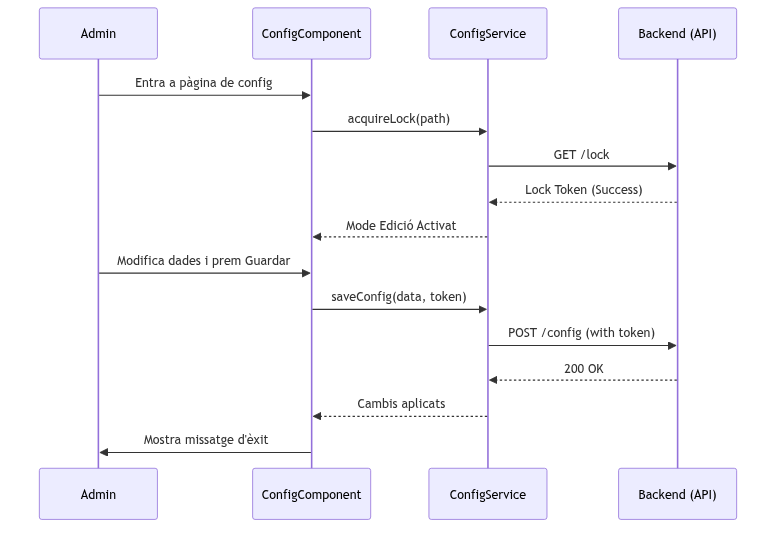
\includegraphics[width=0.9\textwidth]{figures/seq_config_lock.png}
  \caption{Diagrama de seqüència del procés d'adquisició i alliberament de Lock de configuració.}
  \label{fig:seq_config_lock}
  \small Font: Elaboració pròpia.
\end{figure}

Si el recurs està ocupat, el servidor respon amb un codi \texttt{HTTP 409 Conflict} aportant el nom de l'usuari i la IP que té el bloqueig, obligant l'aplicació Angular a bloquejar la vista actual com a "Només lectura" de forma instantània (Figura \ref{fig:seq_config_lock}).

\subsection{Detecció de Deltes i Gestió de Reinicis}
En prémer el botó de desar, en lloc d'enviar tot l'arbre de configuració (el que saturaria el canal d'escriptura i el maquinari del gravador), s'executa l'algorisme recursiu de diferències programat en el frontend (\texttt{getObjectDelta}), comparant l'estat actual contra l'estat inicial original. Les modificacions s'envien mitjançant peticions parcials \texttt{PATCH}:

\begin{lstlisting}[language=JavaScript, caption={Algorisme recursiu de detecció de Deltes per a l'optimització de payloads amb normalització de primitius.}]
export function getObjectDelta(current: any, original: any, path: string = ''): any {
  const normalize = (val: any) => {
    if (val === 'true') return true;
    if (val === 'false') return false;
    return val;
  };

  const normCurrent = normalize(current);
  const normOriginal = normalize(original);

  if (normCurrent === normOriginal) return undefined;
  if (typeof normCurrent !== 'object' || normCurrent === null) return normCurrent;

  const delta: any = {};
  let hasChanges = false;

  for (const key in normCurrent) {
    if (key.startsWith('_')) continue; // Ignora camps estructurals de l'esquema
    
    const currentVal = normCurrent[key];
    const originalVal = normOriginal ? normOriginal[key] : undefined;

    const diff = getObjectDelta(currentVal, originalVal, `${path}.${key}`);
    
    // Evita la propagacio de sub-objectes buits sense canvis reals
    if (diff !== undefined && (typeof diff !== 'object' || Object.keys(diff).length > 0)) {
      delta[key] = diff;
      hasChanges = true;
    }
  }
  
  return hasChanges ? delta : undefined;
}
\end{lstlisting}

Un aspecte de rendiment crític gestionat pel backend és la detecció automàtica de si el canvi d'un d'aquests paràmetres requereix reiniciar l'NVR per aplicar-se (marcat amb la propietat \texttt{\_rebootRequired: true} dins del seu esquema de definició YAML).

Quan s'aplica l'escriptura de dades, el validador del backend avalua si qualsevol camp de la delta conté aquesta bandera. Si és així, el servidor estableix automàticament un indicador global de "Reinicio pendent" i injecta de manera asíncrona la capçalera personalitzada \texttt{X-Reboot-Required: true} a la resposta HTTP de l'API. L'interceptor d'Angular llegeix la capçalera i actualitza l'estat de les vistes, de manera que el frontend sap de forma dinàmica i unificada quan avisar l'operador, sense necessitat de duplicar aquesta lògica de negoci complexa en el codi de la interfície de client.

\section{Assistents de Configuració (Wizards)}
El sistema també disposa d'assistents pas a pas (\textit{Wizards}) per facilitar la posada en marxa ràpida de l'equip a operadors sense coneixements tècnics avançats. S'ha adaptat completament l'estètica CSS de l'eina \textit{legacy} per adequar-la al disseny modern i reactiu de la nova aplicació, guiant l'usuari en la detecció automàtica de càmeres IP a la xarxa local de forma interactiva i assistida.

\section{Eina de Xarxa: Web Proxy}
Atès que, per motius de seguretat, algunes càmeres IP estan connectades a ports aïllats del gravador (creant una subxarxa no accessible des de l'exterior), l'aplicació integra l'eina de \textit{Web Proxy}.

\begin{figure}[htbp]
  \centering
  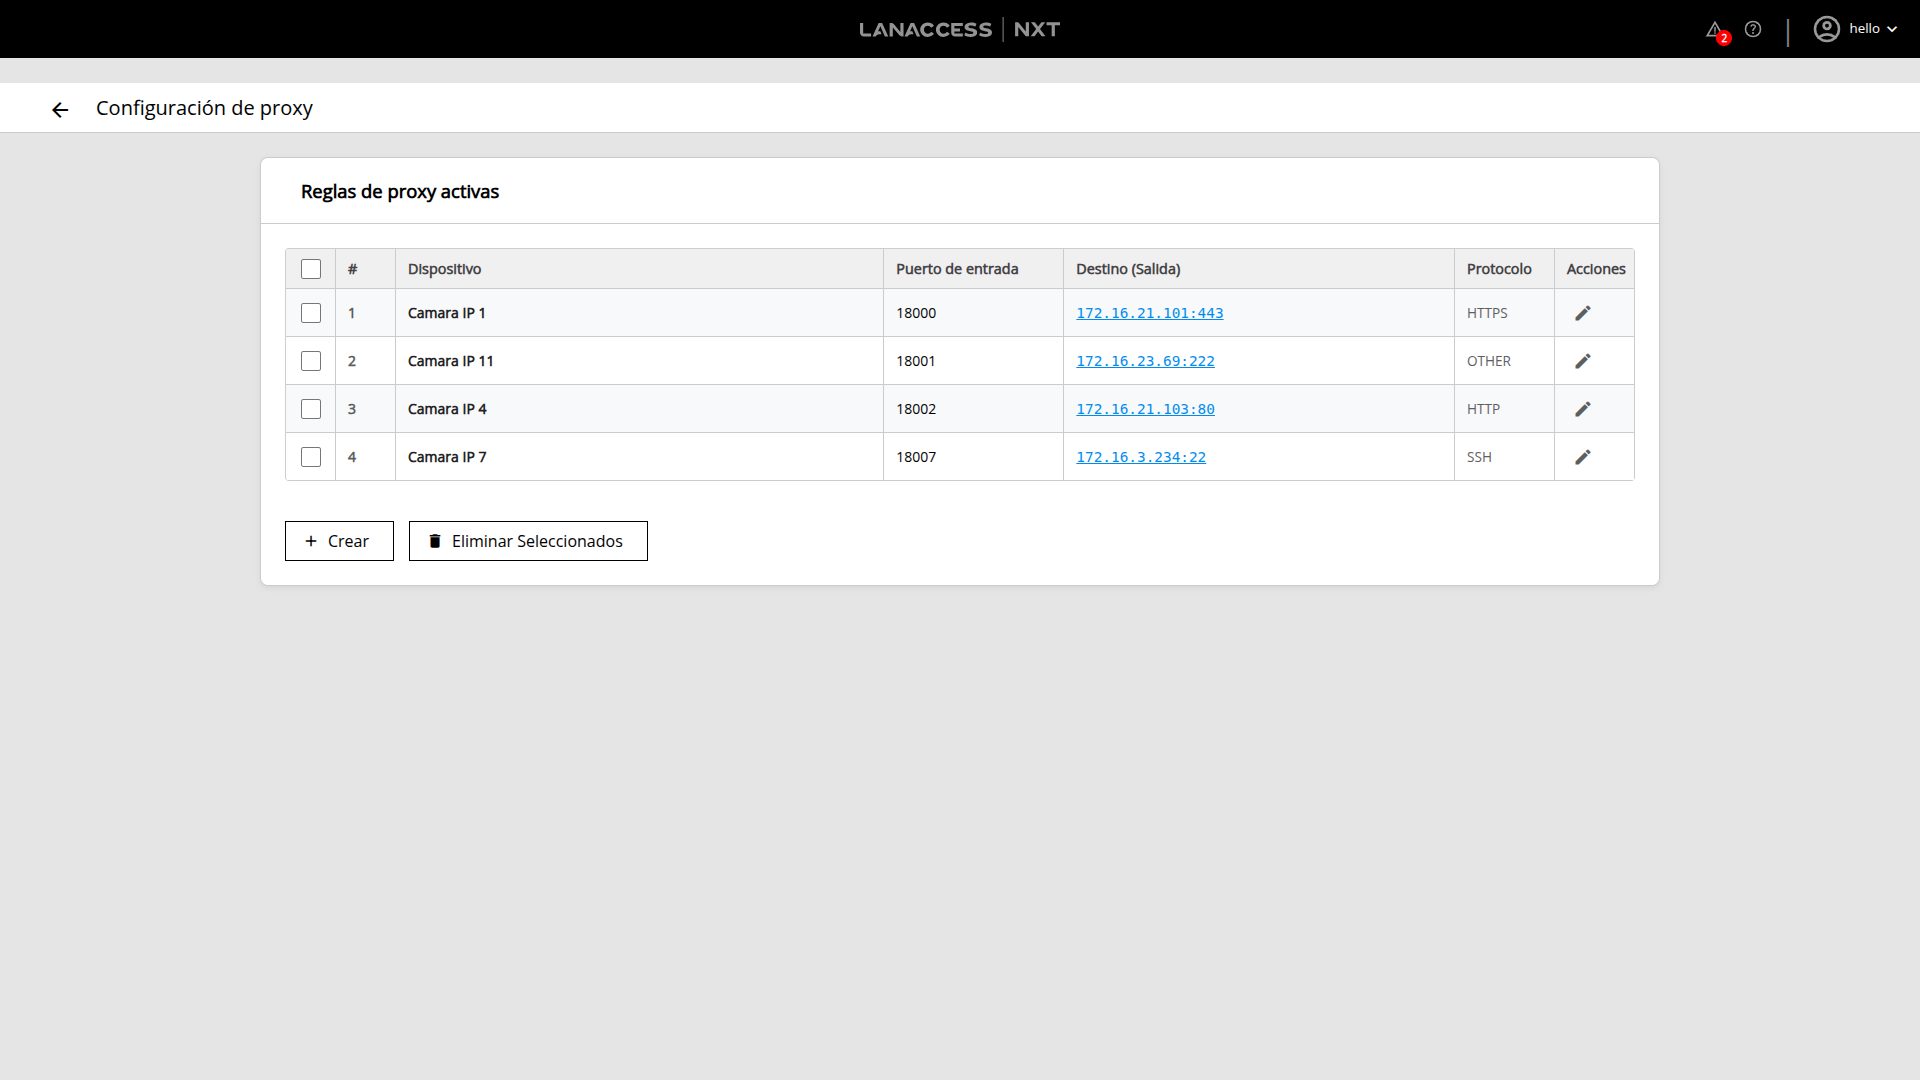
\includegraphics[width=0.95\textwidth]{figures/ui_proxy.png}
  \caption{Eina de Web Proxy per a l'accés a càmeres aïllades en subxarxes internes.}
  \label{fig:ui_proxy}
\end{figure}

Mitjançant aquesta pantalla senzilla (Figura \ref{fig:ui_proxy}), l'administrador pot introduir la IP local de la càmera i el port. El \textit{frontend} es comunica amb \textbf{la-core-legacy} per ordenar la creació d'un túnel invers intern, permetent l'accés al portal web natiu de la càmera des de dins de l'aplicació \textit{Web Core View}.

\section{Visualització Multimèdia en Directe i Arquitectura del Servidor de Vídeo}
La visualització de vídeo en directe representa el component més crític de l'operativa de seguretat diària. Per aconseguir un flux de streaming d'alta fidelitat i eliminar l'ús de connectors externs o codi propietari del costat de client, s'ha implementat una arquitectura híbrida de vídeo integrada al sistema operatiu embedded del gravador NXT, utilitzant el protocol de comunicació estàndard \textbf{WebRTC} com a canal de transport principal i \textbf{HLS} (\textit{HTTP Live Streaming}) com a mètode de contingència o \textit{fallback}.

\begin{figure}[htbp]
  \centering
  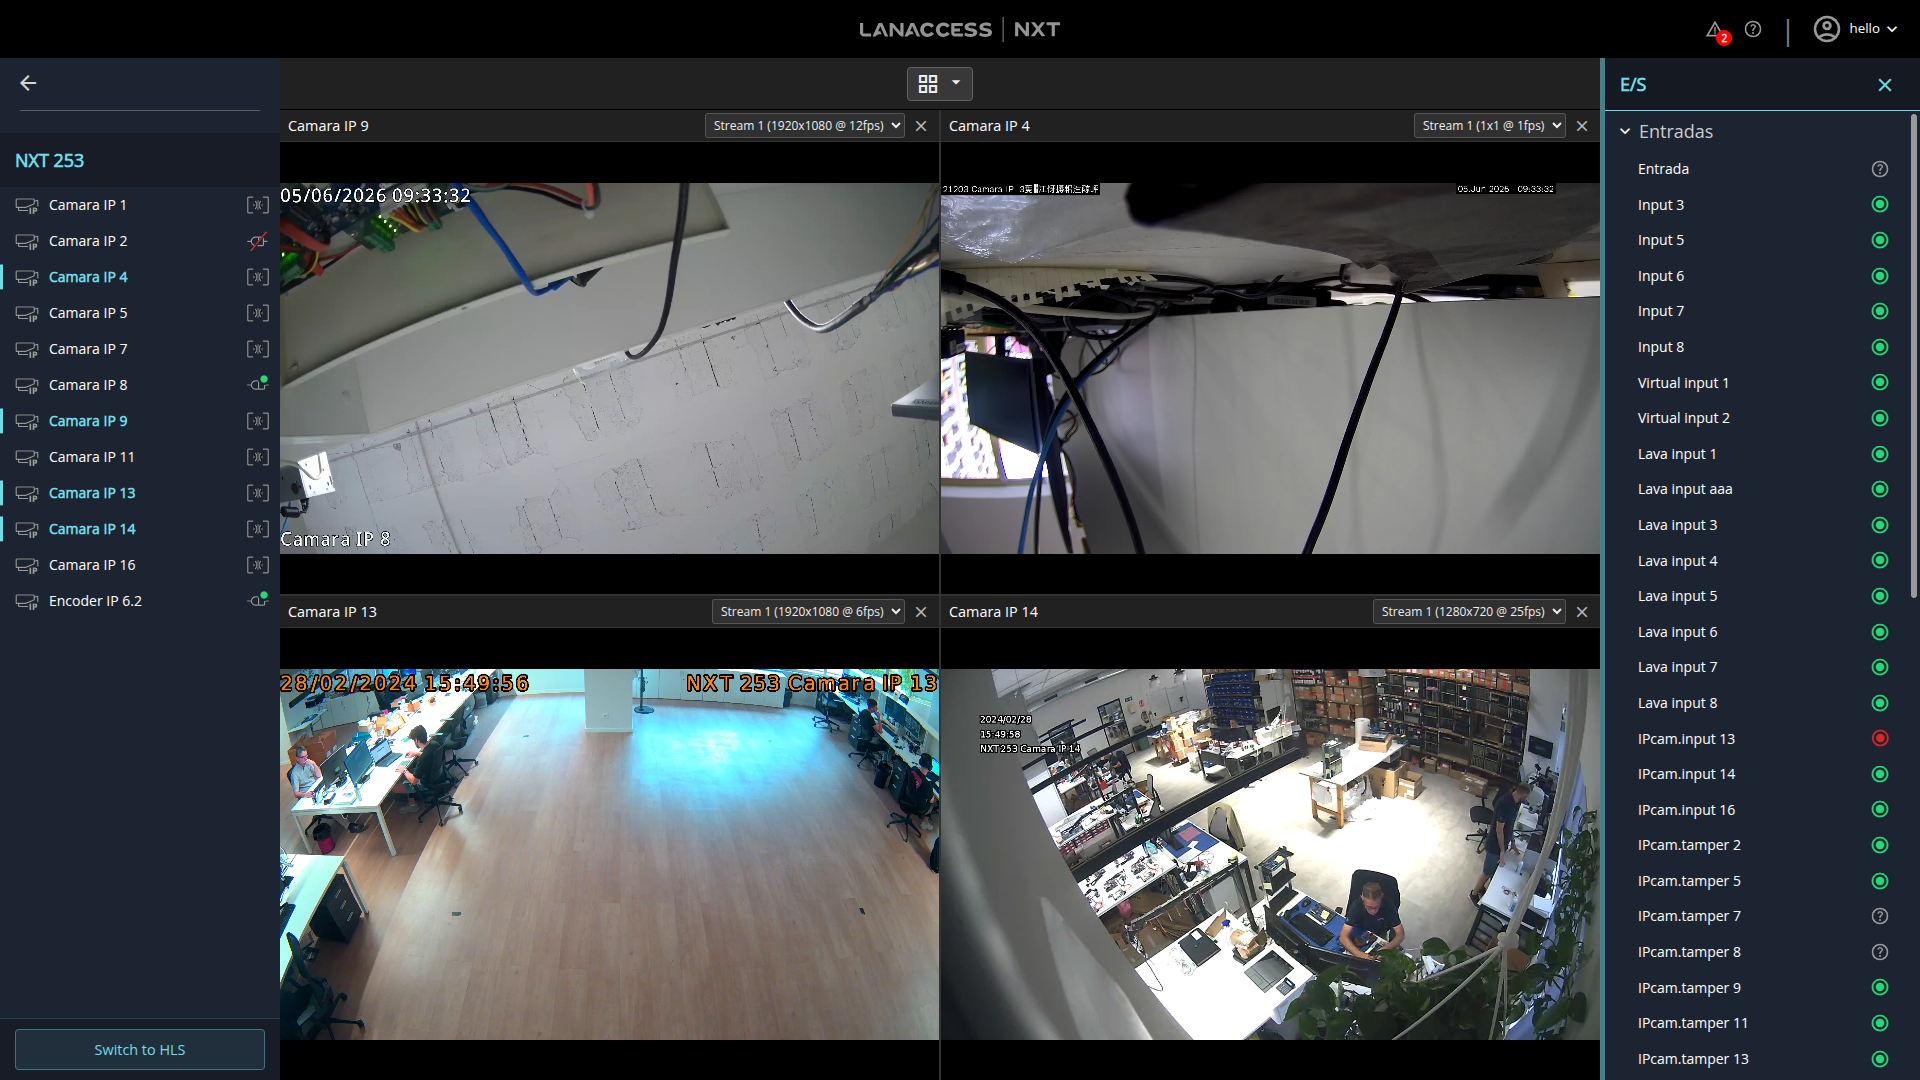
\includegraphics[width=0.95\textwidth]{figures/ui_cameras.png}
  \caption{Mosaic de visualització de vídeo en directe.}
  \label{fig:ui_cameras}
\end{figure}

A nivell de maquinari del gravador, l'arquitectura de transmissió de vídeo es divideix en dues capes diferenciades coordinades pel microservei \textbf{la-video-engine}:

\begin{enumerate}
  \item \textbf{Motor d'Adquisició i Processat (GStreamer):} Per a cadascuna de les càmeres IP físiques instal·lades, l'NVR inicialitza un pipeline de dades basat en el framework multimèdia industrial \textbf{GStreamer}. Aquest pipeline s'encarrega d'obrir el flux \textit{RTSP} natiu de la càmera, extreure'n els paquets de vídeo, normalitzar el senyal de rellotge i decodificar de forma accelerada per maquinari part dels fotogrames crítics per a la generació de metadades analítiques.
  \item \textbf{Servidor de Mitjans WebRTC (MediaMTX):} Els fotogrames de vídeo capturats i empaquetats per GStreamer es canalitzen internament en un pipeline d'escriptura cap al servidor multimèdia d'alt rendiment \textbf{MediaMTX} (actuant com a servidor centralitzat de WebRTC i WHEP). Aquest servei gestiona la negociació SDP (\textit{Session Description Protocol}), el xifratge de paquets SRTP sobre transport UDP, i serveix el vídeo amb una latència punta a punta inferior a 300 ms natius en qualsevol navegador web actual, recolzant-se en la targeta gràfica (GPU) del dispositiu del client per a la descodificació fina.
\end{enumerate}

Davant de xarxes corporatives on el trànsit UDP pugui estar completament bloquejat pel tallafocs de l'empresa (la qual cosa impedeix establir el canal de vídeo per defecte d'ICE), el sistema activa de forma transparent un mecanisme de degradació de servei cap a \textbf{HLS} (\textit{HTTP Live Streaming}). Aquesta via de redundància s'estableix a través del proxy invers NGINX mitjançant el port de comunicació de dades estàndard (TCP 443), assegurant la visualització contínua i sense talls del senyal a costa d'un petit increment de la latència que no excedeix el límit operatiu.

\subsection{La Interfície de Càmeres i el Disseny de Mosaic}
A la pàgina de Càmeres (Figura \ref{fig:ui_cameras}), l'operador disposa de controladors visuals per commutar la distribució de la graella multimèdia (\textit{layouts} de tipus $1\times1$, $2\times2$ i $4\times4$). Cadascuna de les cel·les que formen aquest mosaic és un component d'Angular unificat i encapsulat anomenat \texttt{GridVideoPlayerComponent}, el qual gestiona el cicle de vida del seu propi reproductor independent.

La interfície implementa una lògica d'arrossegar i deixar anar (\textit{Drag and Drop}) nativa integrada amb la llista lateral de càmeres del panell esquerre. L'usuari pot arrossegar qualsevol càmera cap a una cel·la del mosaic. Aquesta acció de drop recupera la identitat del dispositiu d'entrada, demana el seu mètode d'accessibilitat i demana de forma dinàmica la càrrega del flux, seguint el cicle d'activitat descrit a la Figura \ref{fig:activity_video_connection}.

\begin{figure}[htbp]
  \centering
  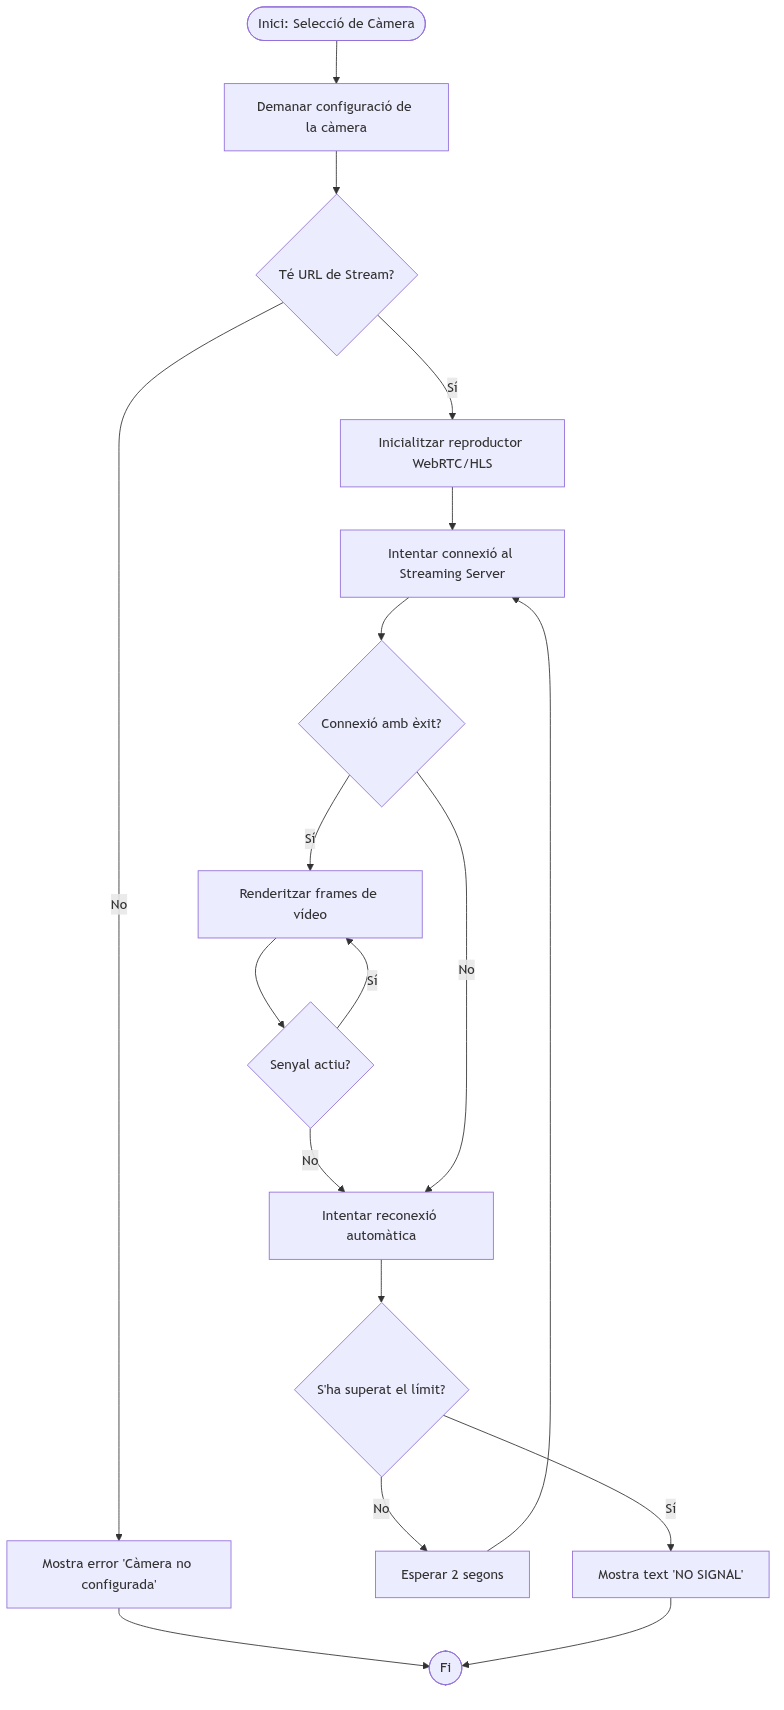
\includegraphics[width=0.65\textwidth]{figures/activity_video_connection.png}
  \caption{Diagrama d'activitat de la lògica de connexió i reconnexió de vídeo.}
  \label{fig:activity_video_connection}
\end{figure}

\subsection{Negociació SDP i Establiment del Canal de Streaming}
Si la xarxa del client disposa dels canals lliures de comunicació, el frontend i el servidor MediaMTX inicien la negociació SDP mitjançant el protocol d'egress de mitjans unificat \textbf{WHEP} (\textit{WebRTC HTTP Egress Protocol}):

\begin{lstlisting}[language=JavaScript, caption={Lògica simplificada de la PeerConnection per WebRTC.}]
async startStreaming(cameraId: string) {
  const pc = new RTCPeerConnection(this.config);
  
  // Generacio de l'oferta local de presentacio
  const offer = await pc.createOffer();
  await pc.setLocalDescription(offer);
  
  // Enviament al servidor MediaMTX a traves de la-video-engine
  this.videoService.sendOffer(cameraId, offer).subscribe(answer => {
    // Aplicacio de la resposta del servidor (Answer) per establir el canal
    pc.setRemoteDescription(answer);
  });
}
\end{lstlisting}

Aquest intercanvi de metadades descrit en el diagrama de seqüència de la Figura \ref{fig:seq_video_streaming} defineix quins còdecs d'escriptura (H.264 o H.265) i resolucions utilitzarà l'enllaç abans d'iniciar el transport segur dels paquets sobre canals UDP.

\begin{figure}[htbp]
  \centering
  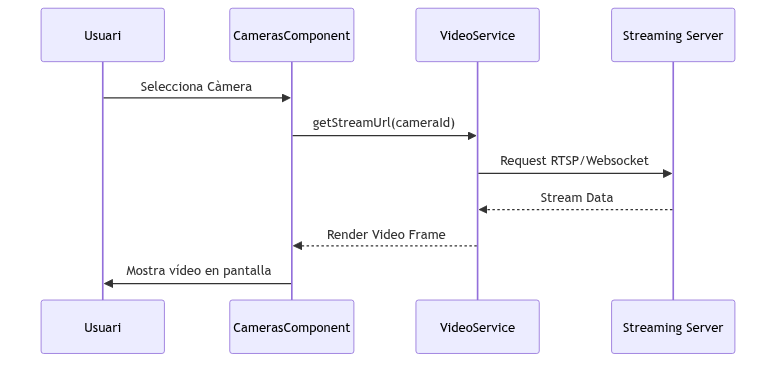
\includegraphics[width=0.85\textwidth]{figures/seq_video_streaming.png}
  \caption{Diagrama de seqüència de l'establiment de streaming de vídeo (SDP).}
  \label{fig:seq_video_streaming}
\end{figure}

\subsection{Orquestració de Vídeo amb el Patró Strategy}
Per estructurar el reproductor multifluj, s'ha aplicat el patró de disseny de programari \textbf{Strategy} d'Angular. Aquest disseny desacobla completament el component visual de la graella de les APIs i llibreries de tercers implicades en la descodificació. Es defineix la interfície comuna \texttt{StreamingStrategy} que actua com a contracte o interfície abstracta unificada:

\begin{lstlisting}[language=JavaScript, caption={Interfície comuna \texttt{StreamingStrategy}.}]
export interface StreamingStrategy {
  connectionState: Signal<'connecting' | 'connected' | 'error' | 'idle'>;
  errorMessage: Signal<string | null>;
  startStream(videoElement: HTMLVideoElement, cameraName: string): Promise<void>;
  closeStream(): void;
}
\end{lstlisting}

Un \textit{InjectionToken} personalitzat allotjat a la declaració del component injecta dinàmicament l'estratègia correcta (ja sigui el servei WebRTC o la via de redundància HLS) en funció de les capacitats obtingudes del mètode de streaming triat:

\begin{lstlisting}[language=JavaScript, caption={Proveïdor per a la injecció dinàmica de l'estratègia de vídeo al \texttt{GridVideoPlayerComponent}.}]
export const STREAMING_STRATEGY_TOKEN = new InjectionToken<StreamingStrategy>('StreamingStrategy');

@Component({
  selector: 'app-grid-video-player',
  // ...
  providers: [
    {
      provide: STREAMING_STRATEGY_TOKEN,
      useFactory: () => {
        const method = getStreamingMethod();
        return method === 'hls' ? inject(HlsService) : inject(WebRTCService);
      }
    }
  ]
})
\end{lstlisting}

Gràcies a l'arquitectura del patró de disseny *Strategy*, el component de visualització és capaç d'intercanviar protocols de transport de manera totalment asíncrona i transparent per a l'usuari en temps de d'execució.

\subsection{Gestió en Temps Real de les Entrades i Sortides Digitals (I/O)}
De forma complementària al panell de visualització de les càmeres de seguretat, la vista principal disposa d'un panell lateral interactiu de control d'entrades i sortides lògiques (I/O), anomenat \texttt{CamerasIoPanelComponent}. Aquest panell permet realitzar la supervisió d'accessos en temps real i accionar relés de manera manual des d'una interfície unificada.

La reactivitat dels indicadors visuals es manté gràcies a l'obertura d'un canal d'esdeveniments unificat via WebSocket d'alta velocitat connectat directament al microservei \textbf{la-core-notifier}. L'arquitectura utilitza l'esquema següent per a la gestió interactiva d'aquests recursos:

\begin{itemize}
  \item \textbf{Supervisió de Canvis (Estat d'Entrada):} El servei escolta el flux del canal i rep el tipus d'esdeveniment \texttt{IO\_NOTIFY}. En rebre la dada, actualitza a l'instant el mètode reactiu de la llista de sensors digital, fent canviar el color de l'indicador del DOM (verd per a \textit{deactivated/idle}, vermell per a \textit{activated/on}).
  \item \textbf{Activació Manual (Estat de Sortida):} Si el perfil de l'operador disposa de permisos de control d'I/O de tipus d'escriptura actius, pot realitzar un doble clic sobre qualsevol de les sortides lògiques configurades, o obrir el menú contextual a través de la icona corresponent.
  \item \textbf{Viatge de Dades:} Aquesta interacció de client desencadena de forma immediata una petició d'escriptura POST unificada cap al servei \textbf{la-core-legacy} sota la ruta \texttt{output-status-set.cgi}. El backend llegeix el camí, valida la intenció i commuta l'estat del relé físic a nivell del maquinari. Un cop realitzat el canvi de sortida, l'NVR llança el senyal de variació a D-Bus, que es propaga a tots els clients connectats a través de WebSocket unificat, garantint la consistència immediata de l'estat global del sistema.
\end{itemize}

\section{Reproducció de Gravacions Històriques i Arquitectura de Playback}
La consulta i reproducció de gravacions passades és un pilar indispensable de l'operativa de seguretat, ja que permet als operadors analitzar i extreure evidències gràfiques d'incidents ja ocorreguts. En el marc d'aquest projecte, s'ha dissenyat i desenvolupat íntegrament tant la capa lògica de negoci del \textit{backend} (l'arquitectura de segmentació, l'indexador de franges de temps i el servidor de mitjans d'HLS integrats al servei \textbf{la-video-engine}) com la interfície interactiva de control del client a Angular 19 (mòdul de \textit{Playback}).

\begin{figure}[htbp]
  \centering
  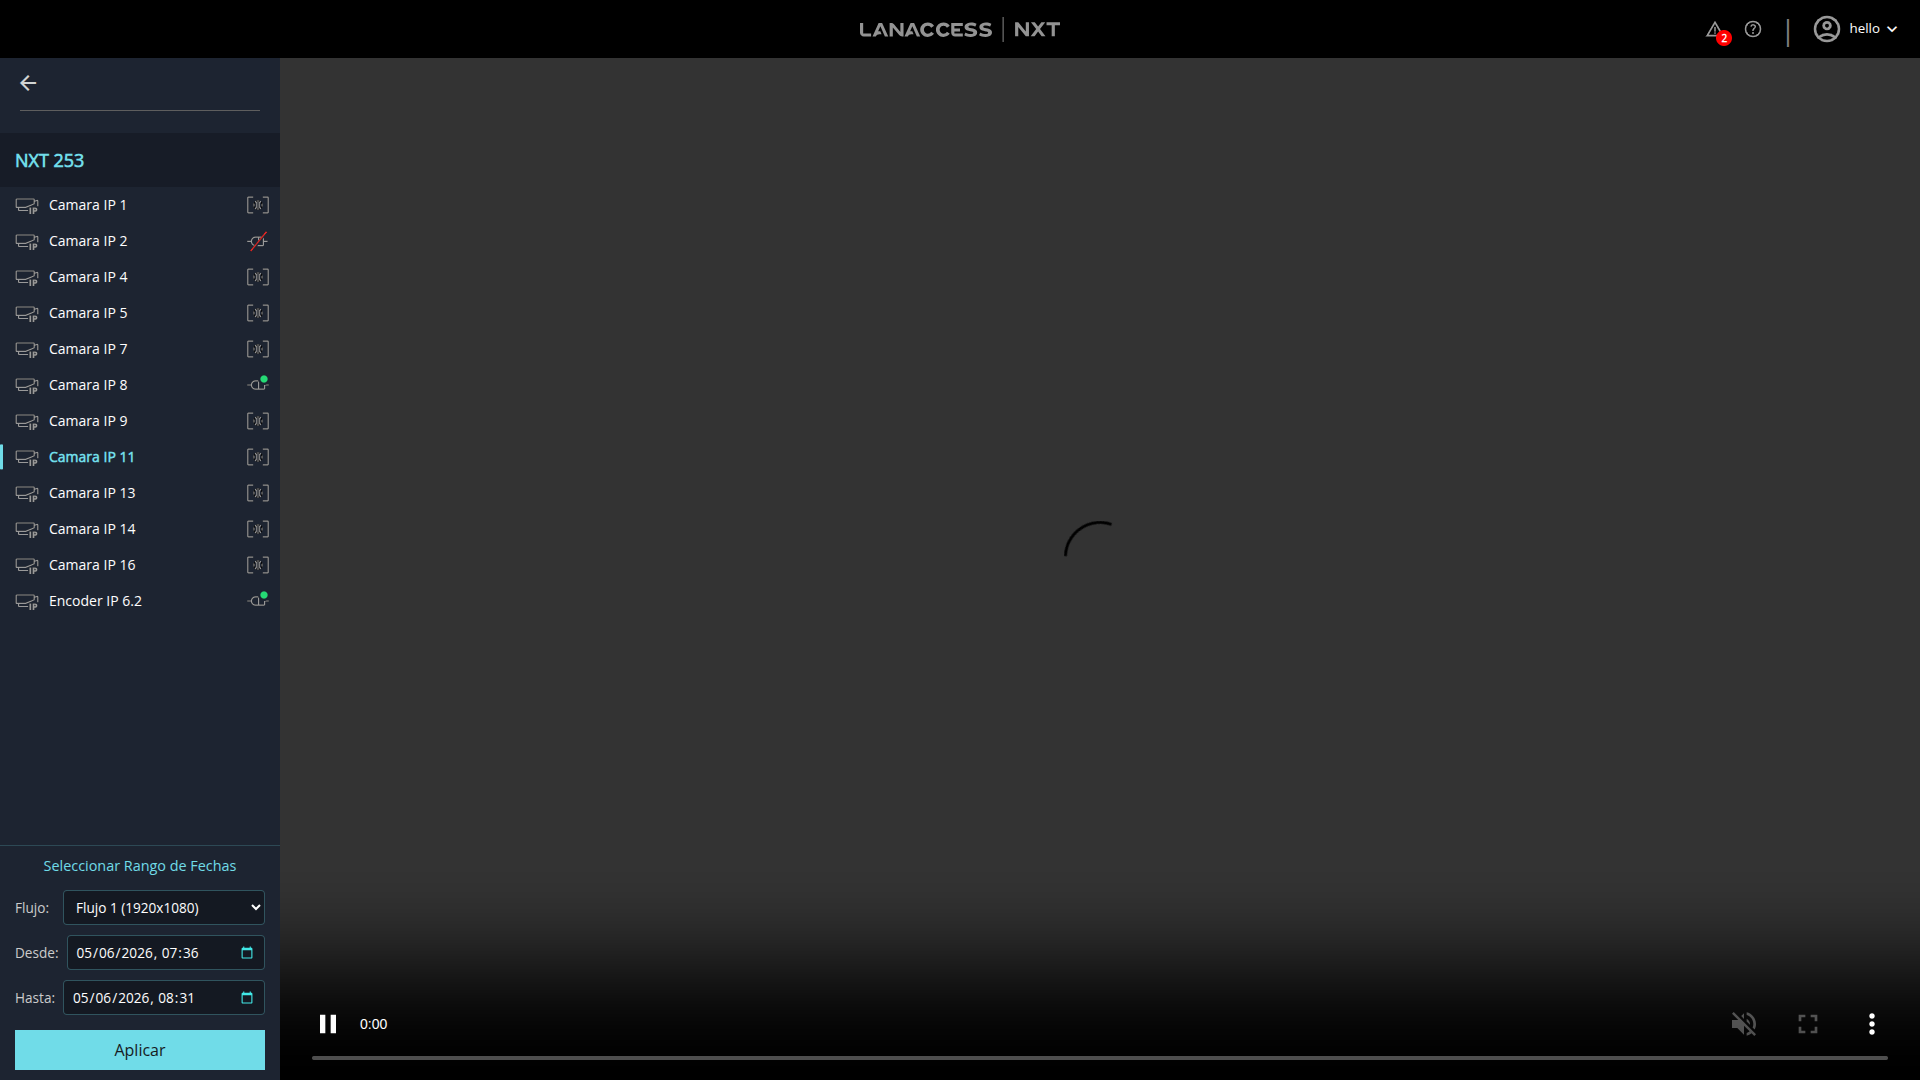
\includegraphics[width=0.95\textwidth]{figures/ui_recordings.png}
  \caption{Vista del reproductor de vídeo històric i component interactiu Timeline.}
  \label{fig:ui_recordings}
\end{figure}

\subsection{El Servidor de Segmentació de Vídeo (la-video-engine Backend)}
El motor de gravacions s'ha dissenyat sota un enfocament de transmissió eficient basat en el protocol estàndard \textbf{HLS} (\textit{HTTP Live Streaming}). El repte tècnic principal del costat del servidor residia en la impossibilitat d'enviar fitxers sencers d'enregistrament degut a l'enorme consum d'ample de banda i memòria RAM que requeriria.

Per resoldre-ho, el microservei \textbf{la-video-engine} (desenvolupat en C++) implementa un pipeline de segmentació multimèdia en temps real que actua sota demanda:
\begin{enumerate}
  \item \textbf{Indexació i Cerca:} Quan el client demana una franja de temps, el servidor interroga directament la base de dades local de l'NVR per localitzar els fitxers d'enregistrament físics afectats.
  \item \textbf{Segmentació Dinàmica (Trans-muxing):} El servidor llegeix els descriptors d'arxiu i, sense realitzar una transcodificació completa (el que sobrecarregaria de manera inacceptable la CPU del gravador), extreu els paquets de vídeo i els empaqueta o encapsula de forma asíncrona en contenidors de transport elementals estàndard MPEG-TS (fitxers \texttt{.ts}) de pocs segons de durada.
  \item \textbf{Generació de Playlist:} El servidor genera un fitxer d'índex o llista de reproducció XML/m3u8 dinàmica (fitxer \texttt{.m3u8}) que apunta a aquests segments temporals virtuals sota un identificador únic o token de sessió temporal de reproducció.
\end{enumerate}

\subsection{El Client de Playback i la Línia de Temps Interactiva (Timeline)}
A l'interfície web (Figura \ref{fig:ui_recordings}), el disseny es divideix en un calendari d'elecció de data, un seccionador de càmeres i una línia de temps interactiva de dades de tipus \textit{Timeline} situada a la part inferior. El cicle de funcionament del frontend segueix els passos següents:

\begin{enumerate}
  \item El client demana l'índex de gravacions per a un dia seleccionat mitjançant el component \texttt{DateTimeRangeSelectorComponent}.
  \item El frontend rep un llistat de metadades amb les franges temporals exactes en què s'ha emmagatzemat vídeo.
  \item El motor de renderitzat dibuixa gràficament la línia de temps utilitzant un codi de colors altament intuïtiu per a l'operador: verd/blau per a gravació de tipus continu, i vermell/taronja per a gravació disparada per un esdeveniment d'alarma o analítica.
  \item En fer clic o desplaçar el lliscador del timeline, el frontend calcula el *timestamp* exacte de destí i demana al segmentador de l'NVR la llista de reproducció específica a través de la crida d'escriptura \texttt{loadVideo()} (vegeu el llistat \ref{lst:hls_load_code}).
\end{enumerate}

\begin{lstlisting}[language=JavaScript, label={lst:hls_load_code}, caption={Càrrega dinàmica de llista de reproducció HLS basada en franges de temps.}]
loadVideo(): void {
  const token = this.selectedToken();
  if (this.hls) {
    this.hls.destroy();
    this.hls = undefined;
  }
  if (!this.videoPlayer || !this.selectedCamera() || !token) return;

  const videoElement = this.videoPlayer.nativeElement;
  const start = Math.floor(this.recordingStartTime().getTime() / 1000);
  const end = Math.floor(this.recordingEndTime().getTime() / 1000);
  
  // Construccio de la URL del segmentador dinamic del la-video-engine
  const hlsUrl = `/video-engine/hls-play.m3u8?token=${token}&start=${start}&end=${end}`;

  if (Hls.isSupported()) {
    this.hls = new Hls({
      maxBufferHole: 4.0,          // Tolerancia a buits de dades
      manifestLoadingTimeOut: 20000 // Temps d'espera de xarxa per al manifest
    });
    this.hls.loadSource(hlsUrl);
    this.hls.attachMedia(videoElement);
    this.hls.on(Hls.Events.MANIFEST_PARSED, () => {
      videoElement.play().catch(err => console.warn('Play prevented', err));
    });
  }
}
\end{lstlisting}

\subsection{Coexistència i Descodificació de Còdecs H.264 i H.265}
Un dels reptes de disseny més rellevants abordat en la programació unificada del frontend i el backend és la compatibilitat asíncrona amb els còdecs d'última generació **H.265 (HEVC)** de manera transparent al costat d'**H.264 (AVC)**.

Tot i que el format H.265 permet reduir a la meitat l'espai necessari als discs durs de gravació de l'NVR per a la mateixa qualitat d'imatge (la qual cosa representa un valor comercial i operatiu enorme), el seu suport de descodificació nativa dins dels navegadors web ha estat històricament molt restringit per qüestions de patents, forçant tradicionalment l'empresa a dependre d'aplicacions locals pesades o controls ActiveX.

Amb el nou disseny, el motor de segmentació \textbf{la-video-engine} preserva el còdec d'origen de l'enregistrament de la càmera durant l'empaquetat del segment TS. Durant l'execució al navegador:
\begin{itemize}
  \item El client web d'Angular detecta de forma transparent les capacitats de descodificació per maquinari de la targeta gràfica (GPU) del dispositiu de l'operador.
  \item Si el dispositiu és modern i el navegador web suporta descodificació HEVC, l'NVR transmet els fragments H.265 directament per maximitzar l'estalvi d'ample de banda.
  \item En cas contrari, o si la càmera utilitzada és antiga, el sistema commuta de manera unificada cap a H.264, oferint una fluïdesa total en qualsevol tipus de terminal i garantint una interfície lliure d'instal·lació de complements externs (*Plugin-free*).
\end{itemize}

\section{Sistema d'Alarmes i Comunicació Asíncrona Multi-capa}
La gestió, notificació i persistència d'esdeveniments d'alarma en temps real constitueix un dels requisits no funcionals més crítics del dispositiu, atès que qualsevol retard o pèrdua de dades compromet la seguretat de la instal·lació. En el marc d'aquest projecte, s'ha dissenyat i desenvolupat íntegrament una solució de comunicació multi-capa extrem a extrem: des del model de subscripció reactiva al \textit{frontend} d'Angular 19, passant per les passarel·les de WebSockets d'alta velocitat, fins a arribar al sistema de persistència transaccional de baix nivell al sistema operatiu embedded de l'NVR.

Per tal de conceptualitzar aquest flux d'informació complex, a continuació es descriu la topologia del canal de persistència i propagació d'alarmes des del maquinari fins a la base de dades i l'interfície gràfica d'usuari (UI):

\begin{center}
  \small
  \texttt{[Maquinari/Càmeres]} $\rightarrow$ \texttt{[D-Bus]} $\rightarrow$ \texttt{[la-core-alarm]} $\xrightarrow{\text{gRPC}}$ \texttt{[la-db-engine (VFS Driver)]} \\
  $\xrightarrow{\text{Unix Socket}}$ \texttt{[la-video-engine]} $\xrightarrow{\text{Escriptura}}$ \texttt{[Disc Físic (SQLite3)]} \\
  $\xleftarrow{\text{Lectura/WSS}}$ \texttt{[la-core-notifier / NGINX]} $\xleftarrow{\text{Observable Shared}}$ \texttt{[Frontend Angular 19]}
\end{center}

\subsection{Disseny de Persistència: El Virtual File System (VFS) i Unix Sockets}
Per garantir la transaccionalitat i robustesa de les alarmes (propietats ACID) davant de talls d'energia sobtats, s'ha utilitzat el motor de bases de dades relacional \textbf{SQLite3}. No obstant això, per complir amb les directives de seguretat de sistemes crítics i evitar conflictes de concurrència d'accés a disc (fitxers blocats), s'ha implementat un mètode de persistència altament desacoblat:

\begin{enumerate}
  \item \textbf{El servei d'orquestració (\texttt{la-db-engine}):} Aquest microservei actua com a gestor de la base de dades de dades, de la lògica de consultes SQL i de la comunicació cap al servei d'alarmes mitjançant crides binàries d'alt rendiment \textbf{gRPC}. Tanmateix, per política de seguretat, aquest procés està aïllat en un espai d'usuari (\textit{sandbox}) i no té permisos d'escriptura directa sobre el disc dur.
  \item \textbf{El Driver de VFS Personalitzat:} Per resoldre aquesta restricció, es va dissenyar i registrar un driver de fitxers virtuals personalitzat o **Virtual File System (VFS)** de SQLite3 dins del codi de \texttt{la-db-engine}. Aquest driver intercepta qualsevol crida del motor de la base de dades que requereixi realitzar una escriptura física a disc (com un *commit* de transacció de nova alarma).
  \item \textbf{La Passarel·la per Unix Sockets:} En lloc d'intentar obrir el fitxer de base de dades local, el driver VFS serialitza el bloc d'operacions d'E/S i el transmet immediatament a través d'un canal de comunicació entre processos (IPC) de tipus **Unix Domain Socket** cap al servei \textbf{la-video-engine} (l'únic dimoni del sistema autoritzat a interactuar directament amb la controladora de disc d'emmagatzematge). El motor de vídeo rep els canvis, aplica les regles i realitza l'escriptura persistent de manera absolutament transparent per al motor de base de dades.
\end{enumerate}

\subsection{Optimització del Frontend i Consum de Sockets}
Per al control dels esdeveniments en temps real des de la interfície de client, s'ha implementat un canal de \textbf{WebSockets Segurs (WSS)} unificat mitjançant el patró de disseny **Observer**.

A nivell de client, l'obertura de túnels de comunicació és una operació costosa per a la CPU del gravador embedded i per al servidor d'NGINX. Per evitar que cada component d'interfície o element del DOM que demani dades en temps real (com el mosaic de vídeo, la taula d'alarmes o l'indicador de la capçalera) obri una connexió independent cap a \texttt{la-core-notifier}, s'ha programat un **servei de missatgeria unificat** sota el patró \textit{Observable Shared} (vegeu la Figura \ref{fig:ui_alarms}).

\begin{figure}[htbp]
  \centering
  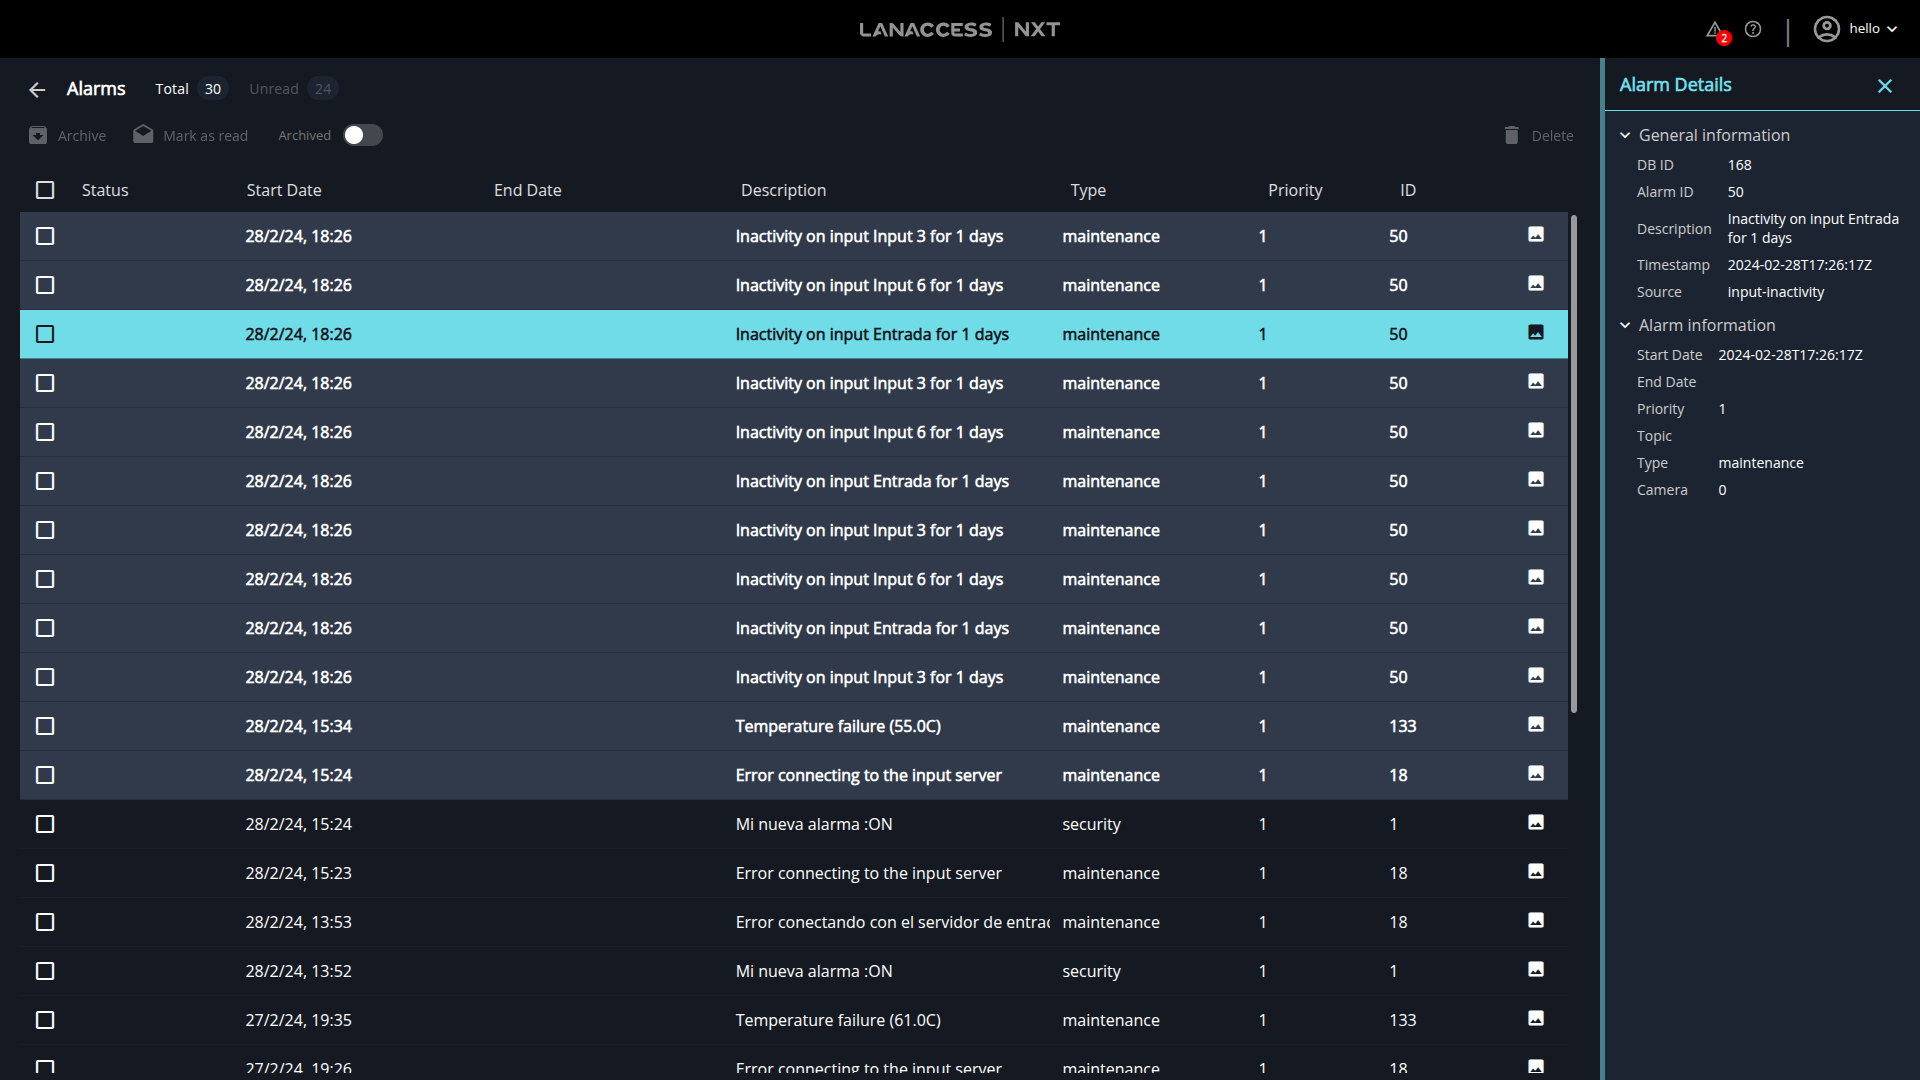
\includegraphics[width=0.95\textwidth]{figures/ui_alarms.png}
  \caption{Taula de monitoratge d'alarmes en temps real i botons d'assentiment.}
  \label{fig:ui_alarms}
\end{figure}

Mitjançant la utilització del pipeline d'RxJS i l'operador \texttt{shareReplay({bufferSize: 1, refCount: true})}, els diferents components de l'aplicació s'acoblen com a subscriptors actius d'una única connexió compartida. L'obertura de sockets es redueix exactament a un canal, el qual es tanca de manera automàtica quan l'usuari surt de les seccions asíncrones de l'aplicació, optimitzant el rendiment global de la memòria de l'equip de xarxa.

\subsection{El Cicle de Vida de l'Alarma i la Robustesa davant de Talls}
Quan el client d'Angular rep un missatge d'esdeveniment a través del canal, l'estat global s'actualitza immediatament, fent que la taula d'alarmes es redibuixi de manera reactiva mitjançant l'ús de \textbf{Signals}. Les alarmes passen per un cicle d'estats descrit a la Figura \ref{fig:state_alarm}:

\begin{figure}[!htbp]
  \centering
  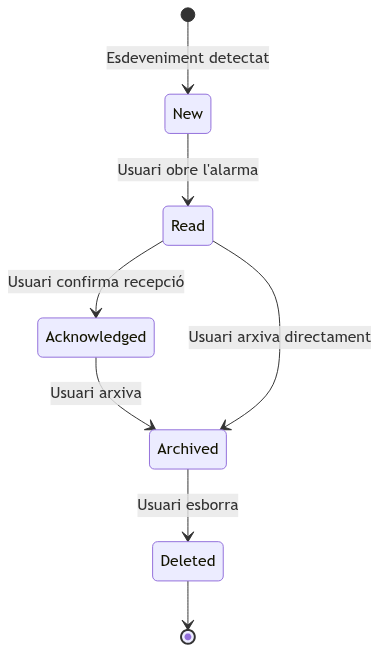
\includegraphics[width=0.55\textwidth]{figures/state_alarm.png}
  \caption{Diagrama d'estats del cicle de vida de les alarmes.}
  \label{fig:state_alarm}
\end{figure}

L'operador pot interaccionar amb cadascun dels incidents per tal d'assentir-los (\textit{Acknowledgment}) fent clic sobre el botó \textit{Ack} al final de la fila. Aquesta operació tanca l'estat actiu de la incidència lògica a l'NVR i silencia el led vermell físic de la placa del videogravador.

Per garantir la continuïtat del servei d'alertes en entorns de xarxa inestables o davant d'interrupcions temporals de la connectivitat del client, la connexió s'ha programat amb una lògica de **reconnexió i Backoff Exponencial** asíncrona:

\begin{lstlisting}[language=JavaScript, caption={Connexió WebSocket resilient amb backoff exponencial en RxJS.}]
this.socket$.pipe(
  retry({
    delay: (error, retryCount) => {
      // 1. Si l'usuari perd la seva sessio, avorta els intents de reconexio
      if (!this.userService.isAuthenticated()) {
        return throwError(() => new Error('Connexio tancada per perdua de credencials.'));
      }
      
      // 2. Incrementa de manera exponencial el temps d'espera per evitar DoS al NVR
      const nextDelay = RECONNECT_INTERVAL_MS * retryCount;
      console.warn(`[WS] Connexio perduda. Intentant reconexio #${retryCount} en ${nextDelay}ms.`);
      return timer(nextDelay); 
    },
  })
).subscribe({
  next: (message) => this.messagesSubject$.next(message)
});
\end{lstlisting}

Aquest disseny asíncron evita que, davant d'un tall generalitzat de xarxa, centenars de clients inundin simultàniament la CPU del videogravador embedded amb peticions agresives de reconnexió, espaiant de manera intel·ligent les cerques fins a restaurar l'estat segur amb el component unificat d'error de connexió.

\subsection{Estructures de Missatges del Canal Asíncron (WebSockets)}
Per documentar el rigor de la integració, a continuació es detallen els missatges JSON que viatgen a través d'aquest servei de notificacions unificat.

El primer missatge que s'envia (Client $\rightarrow$ Servidor) serveix per inicialitzar i subscriure's només a la telemetria desitjada, estalviant amplada de banda:
\begin{lstlisting}[language=json, caption={Missatge d'inicialització del filtre de subscripció.}]
{
  "type": "filter_update",
  "transactionId": "home-page-filter-2026-03-30/12:00:00.123",
  "payload": {
    "include_topics": ["device/notification", "io"]
  }
}
\end{lstlisting}

Quan una entrada digital canvia el seu estat físic, el servidor envia automàticament la notificació següent (Servidor $\rightarrow$ Client):
\begin{lstlisting}[language=json, caption={Notificació asíncrona de canvi d'estat d'E/S.}]
{
  "event": "IO_NOTIFY",
  "payload": [
    {
      "id": "01",
      "idr": "01",
      "data": "on",
      "time": "2026-03-30T12:01:15Z",
      "topic": "io/input"
    }
  ]
}
\end{lstlisting}

Finalment, en el cas de rebre una alarma crítica des de la base de dades (com una intrusió generada des de \textbf{la-core-alarm}), el format inclou totes les metadades persistides a SQLite3:
\begin{lstlisting}[language=json, caption={Notificació d'alarma en temps real de la base de dades.}]
{
  "event": "DB_ENGINE_ALARM_NOTIFY",
  "payload": [
    {
      "alarm_id": "AL_05",
      "db_id": "1054",
      "description": "Intrusio Zona Nord",
      "priority": "1",
      "source": "Camera 3",
      "start_date": "2026-03-30T12:05:00Z",
      "end_date": "-",
      "status": "active",
      "timestamp": "1711800300",
      "topic": "db/alarms",
      "type": "security",
      "camera_num": "3",
      "is_read": false,
      "is_archived": false,
      "is_locked": false
    }
  ]
}
\end{lstlisting}

\section{Manteniment i Gestió de la Infraestructura del Maquinari}
El darrer bloc operatiu d'aplicació d'enginyeria de la plataforma engloba les funcionalitats administratives de suport, dissenyades per allargar la vida útil, facilitar el diagnòstic remot, garantir la traçabilitat de les accions i mantenir la integritat lògica del videogravador. Aquest conjunt d'eines s'ha programat íntegrament en el client d'Angular 19 i es comunica directament amb les APIs d'administració de \textbf{la-core-legacy} i \textbf{la-video-engine}.

\subsection{Mòdul d'Actualització Remota del Firmware}
L'actualització de firmware és un procés crític en sistemes embedded de seguretat, ja que una fallida d'alimentació o d'escriptura durant el procés d'escriptura (\textit{flashing}) pot deixar el dispositiu inutilitzable. Per minimitzar aquest risc i proporcionar una monitorització en temps real a l'operador, s'ha dissenyat un sistema d'actualització robust i tolerant a fallides estructurat en tres fases d'execució:

\begin{figure}[htbp]
  \centering
  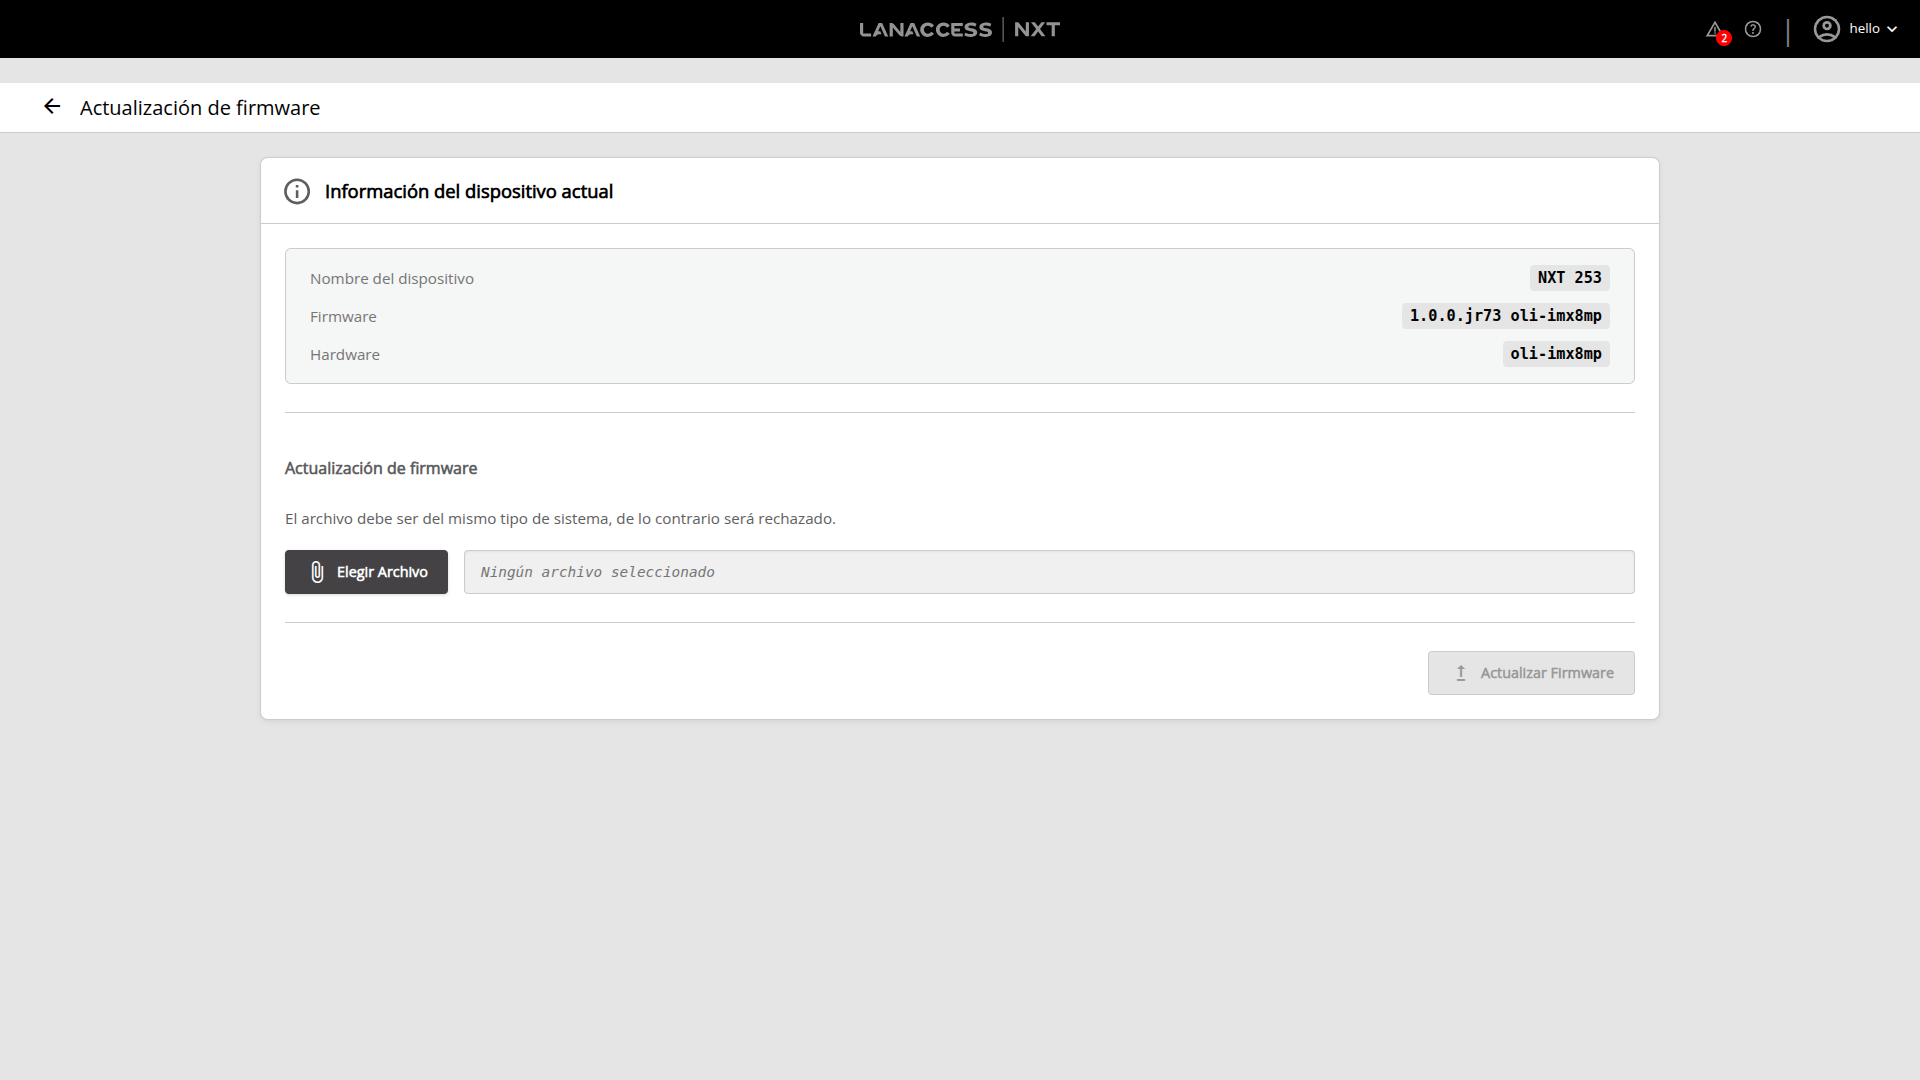
\includegraphics[width=0.95\textwidth]{figures/ui_update.png}
  \caption{Mòdul d'actualització per seleccionar arxius de firmware.}
  \label{fig:ui_update}
\end{figure}

\begin{enumerate}
  \item \textbf{Càrrega i Validació (Figura \ref{fig:ui_update}):} L'operador selecciona el fitxer binari d'actualització (\texttt{.bin}). El frontend valida en primer lloc la firma, l'extensió i la mida del fitxer al navegador abans d'iniciar una petició POST d'escriptura multipart cap a l'endpoint de \texttt{la-core-legacy}.
  \item \textbf{Sondeig d'Estat (\textit{Polling} de Flashing):} Un cop completada la pujada del fitxer, l'aplicació web inicia un procés de consulta periòdica de l'estat cap a \texttt{/webprotocol/firmware\_upgrade\_state} (vegeu la Figura \ref{fig:ui_updating_prog}). L'aplicació mapeja l'estat rebut a la barra de progrés reactiva:
        \begin{itemize}
          \item \texttt{UPLOADING / WAITING:} El fitxer s'està transferint i validant internament.
          \item \texttt{UPDATING:} El sistema està escrivint el nou binari a la partició de firmware secundària des de la memòria d'emmagatzematge temporal.
          \item \texttt{REBOOTING:} S'ordena el reinici del sistema físic.
          \item \texttt{ERROR / INCONSISTENT:} El procés es cancel·la a causa de dades corrompudes o errors de xarxa, activant immediatament la lògica de retorn segur a la partició anterior (\textit{dual-boot rollback}).
        \end{itemize}
  \item \textbf{Recuperació de la Connectivitat (Figura \ref{fig:ui_updating_reboot}):} Quan s'inicia el reinici físic del gravador, l'aplicació web bloqueja la interfície amb una pantalla d'espera i s'absté de fer peticions durant 15 segons de marge segur. Transcorregut aquest temps, inicia un procés de consulta ràpida de la connectivitat IP de xarxa (\texttt{connectivity.cgi}). Un cop restablerta la connexió, es verifica l'èxit definitiu de l'operació preguntant l'estat lògic final, i es permet l'accés un altre cop a la interfície.
\end{enumerate}

\begin{figure}[htbp]
  \centering
  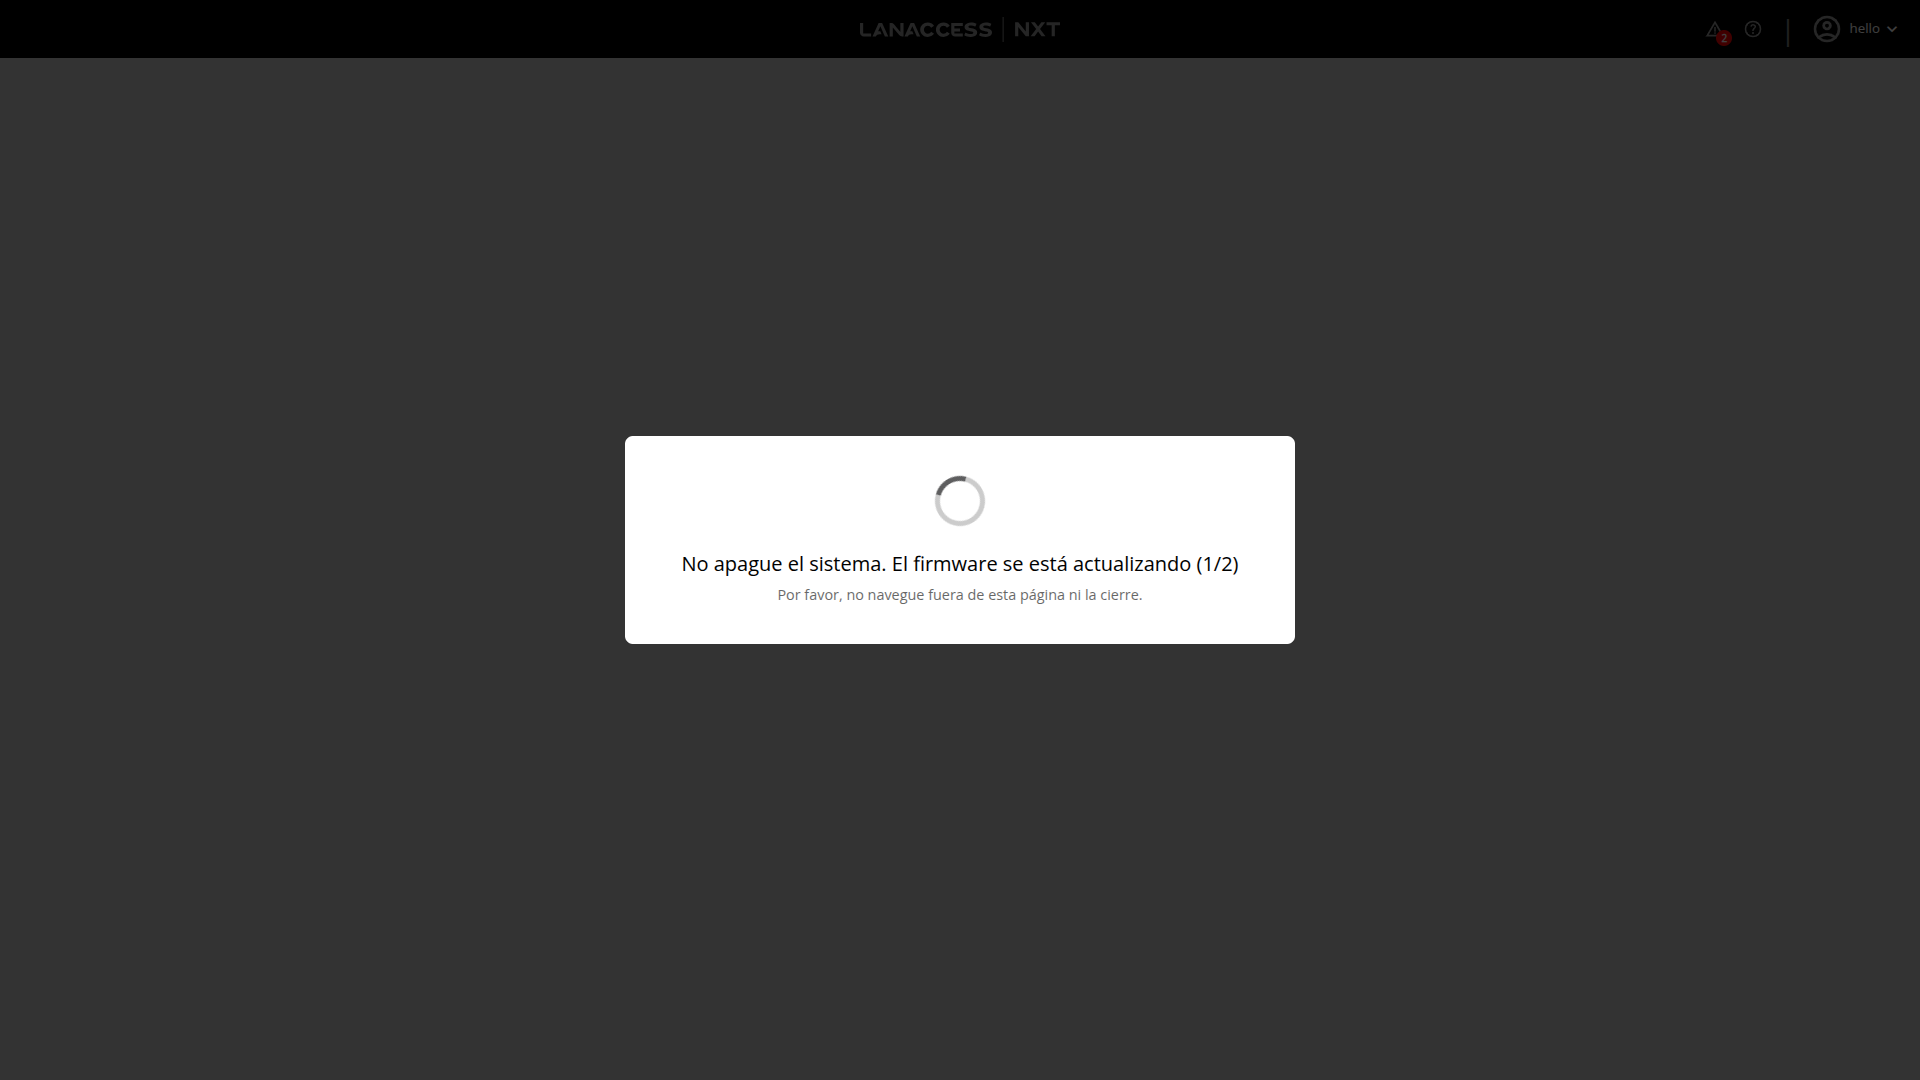
\includegraphics[width=0.48\textwidth]{figures/ui_updating1.png}
  \hfill
  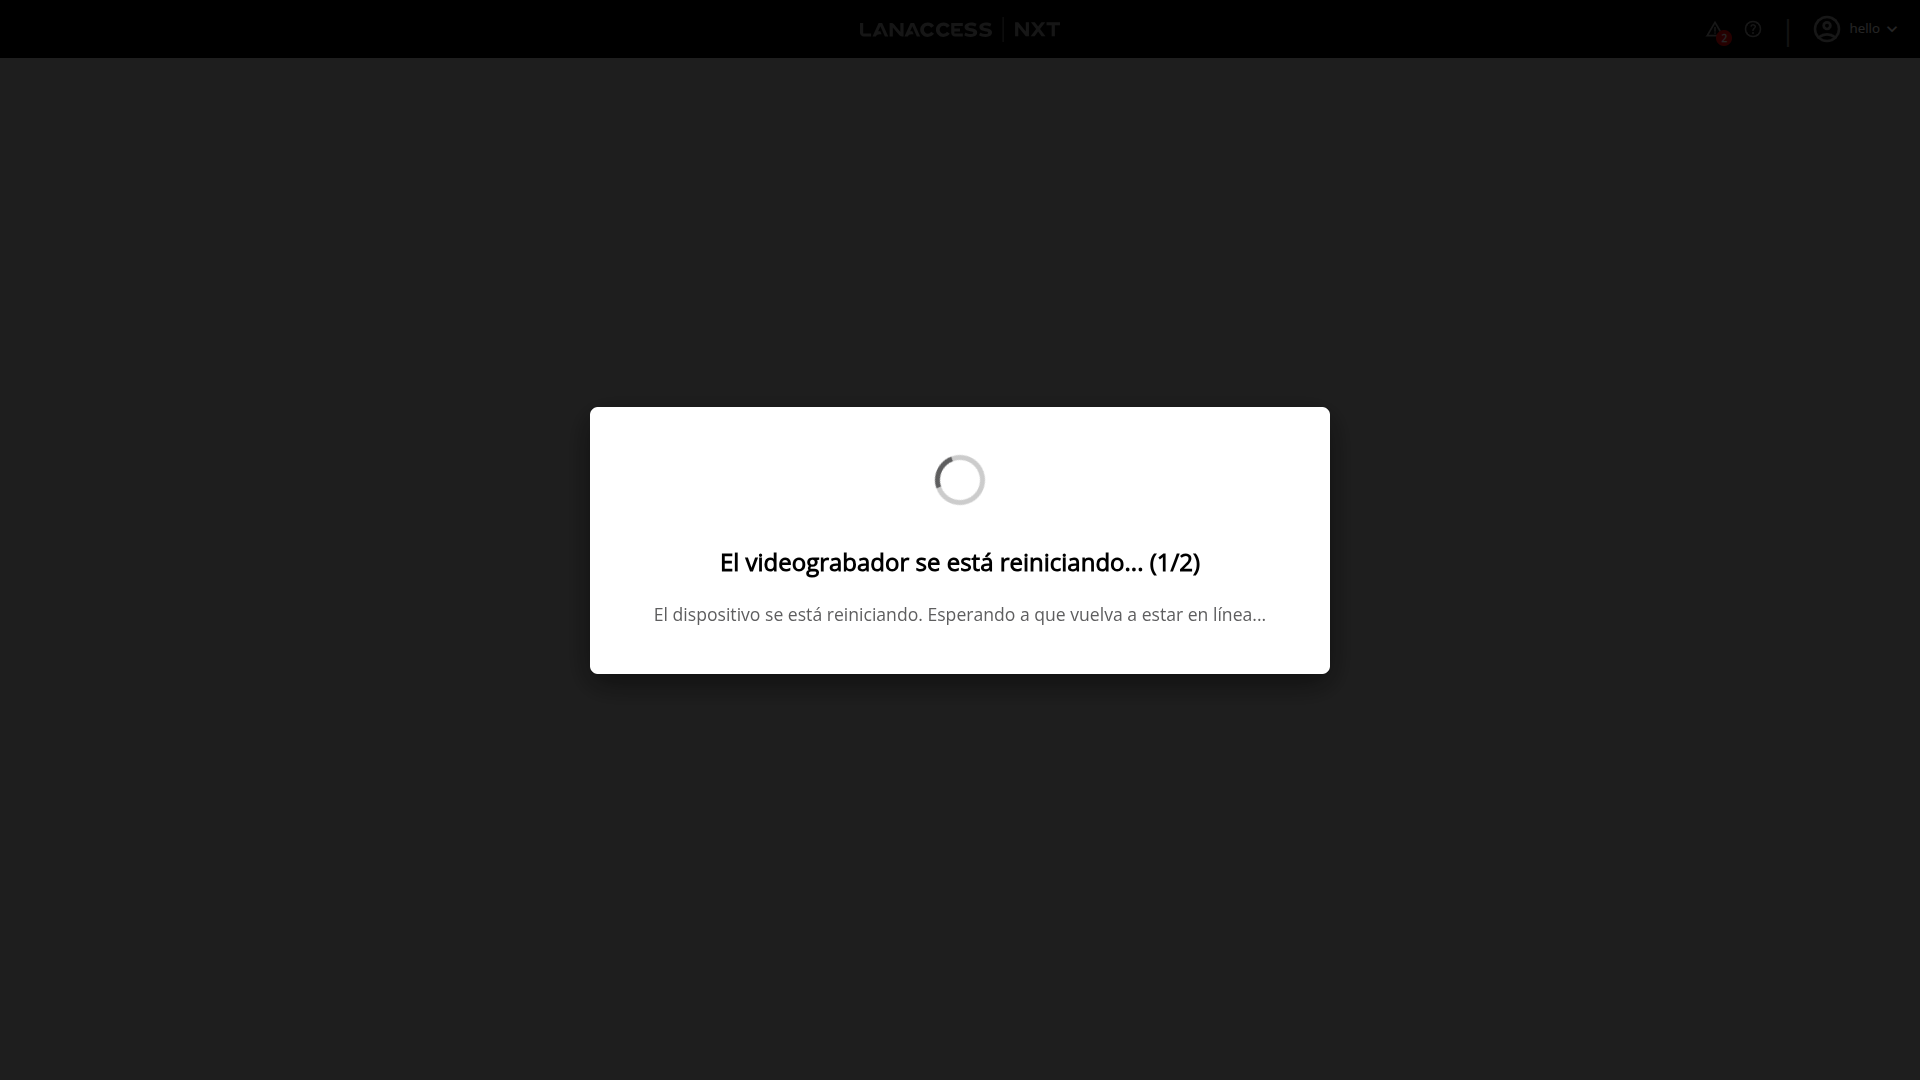
\includegraphics[width=0.48\textwidth]{figures/ui_updating2.png}
  \caption{Barra de progrés reactiva i fases d'escriptura (\textit{flashing}).}
  \label{fig:ui_updating_prog}
\end{figure}

\begin{figure}[htbp]
  \centering
  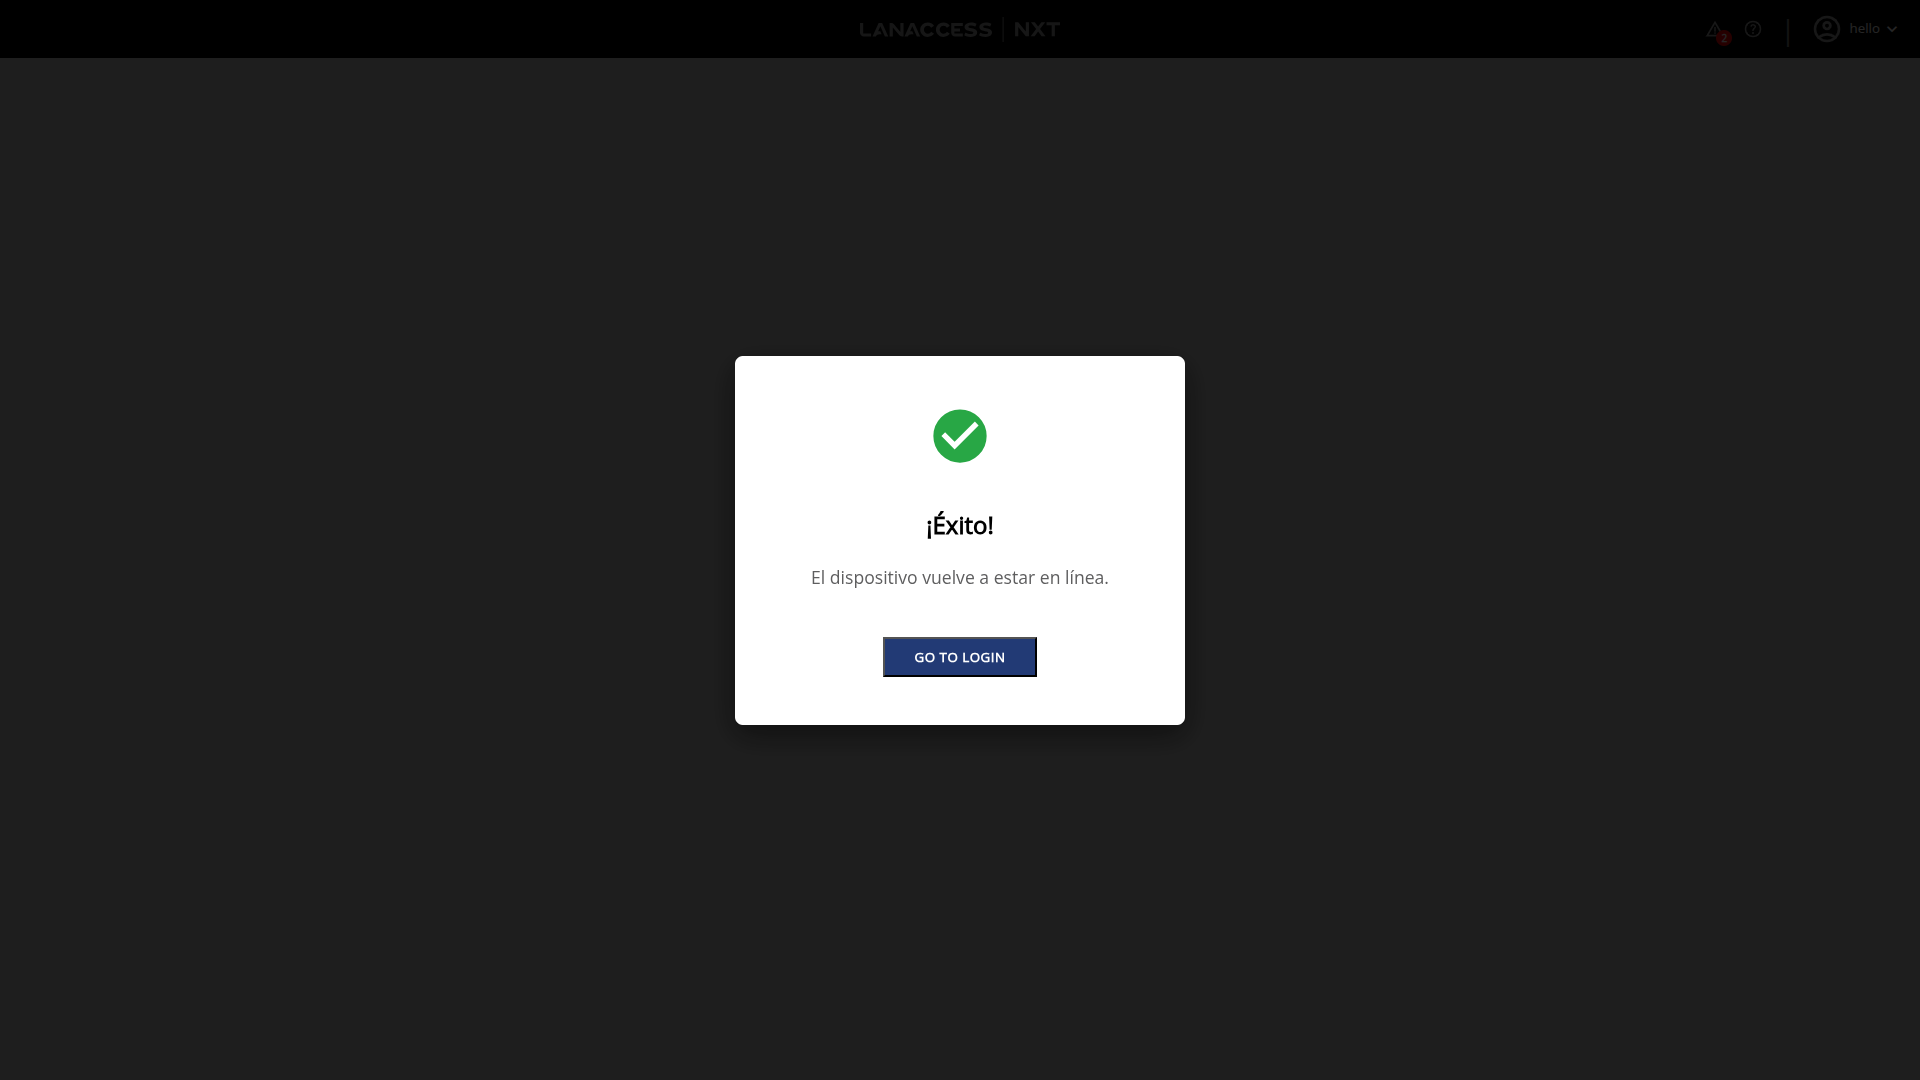
\includegraphics[width=0.95\textwidth]{figures/ui_updating3.png}
  \caption{Pantalla de reinici automàtic amb poldeig de reconnectivitat.}
  \label{fig:ui_updating_reboot}
\end{figure}

\subsection{Mòdul d'Accions Globals: Còpies de Seguretat i Restauració de Fàbrica}
El panell d'accions de configuració unifica les comandes administratives destructives i de salvaguarda de dades (Figura \ref{fig:ui_configuration_actions}).

\begin{figure}[htbp]
  \centering
  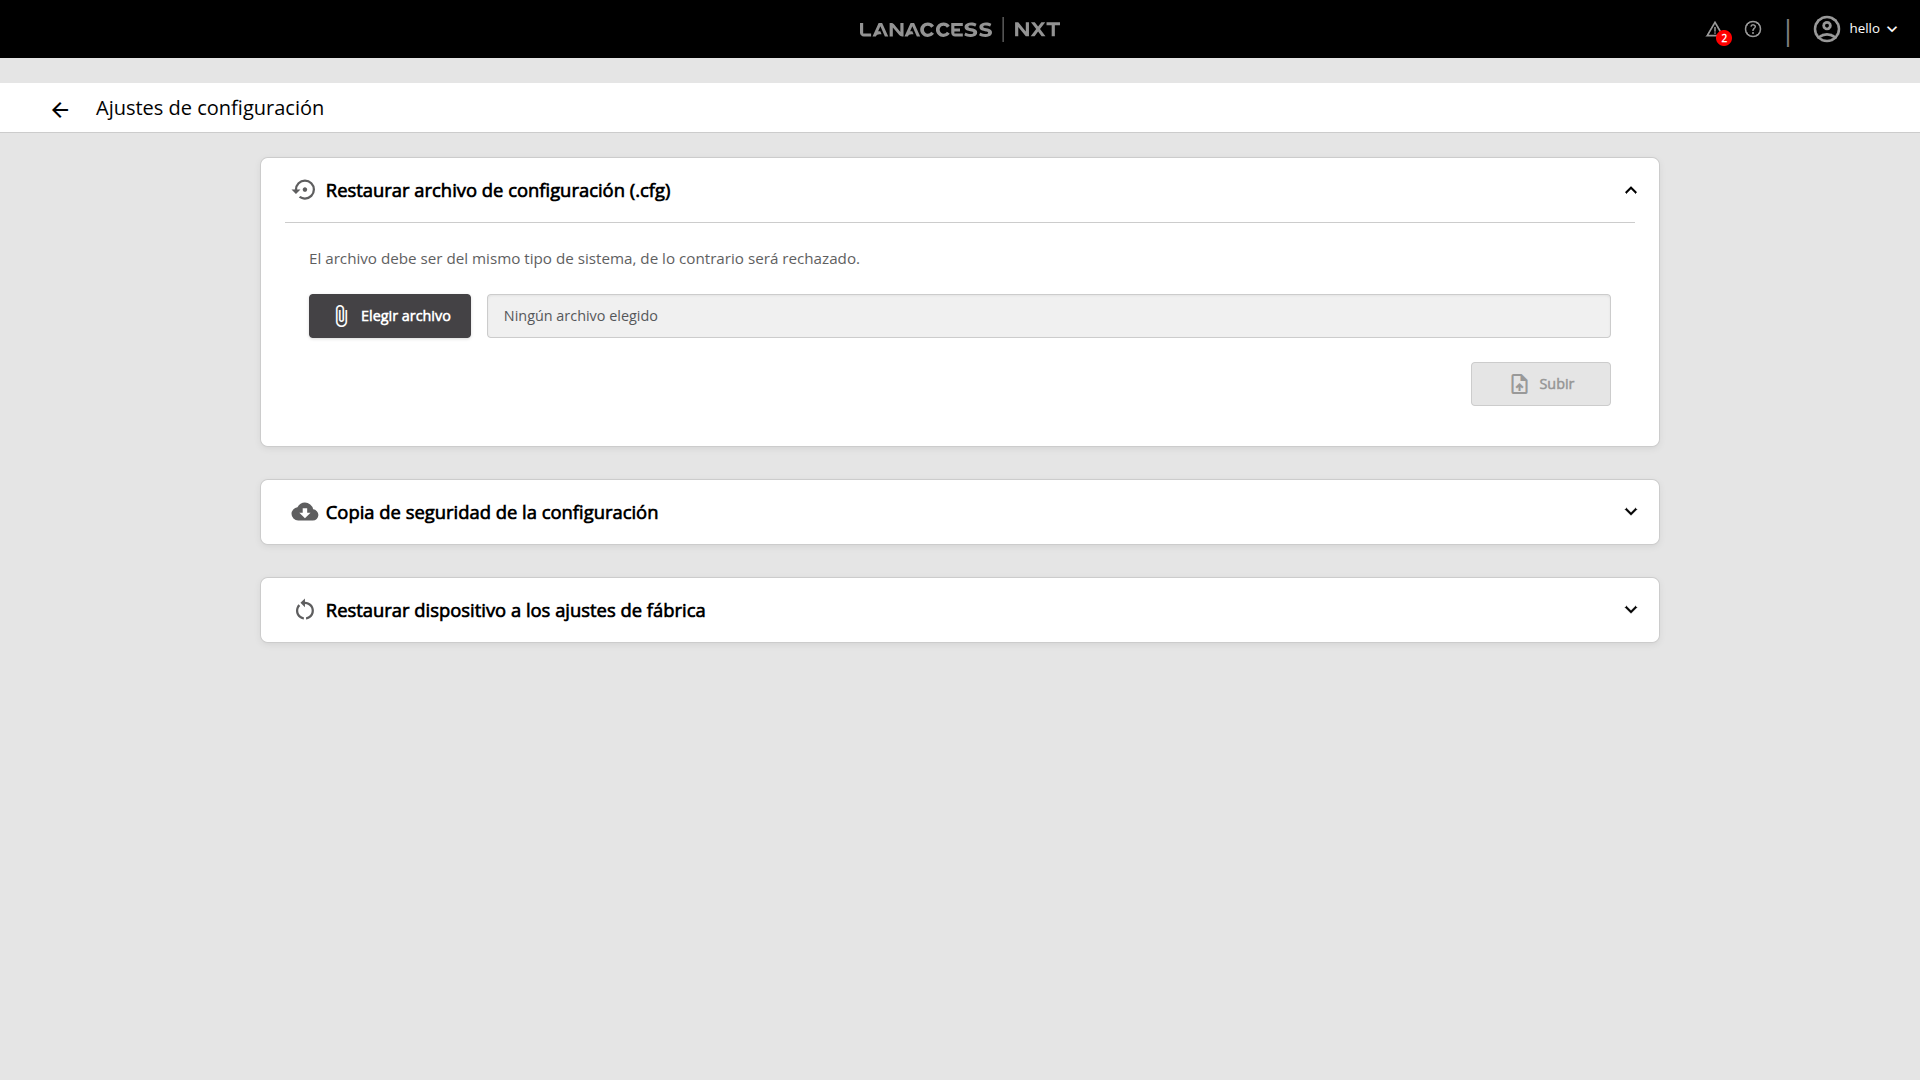
\includegraphics[width=0.95\textwidth]{figures/ui_configuration.png}
  \caption{Accions globals de manteniment: Backup, Restore i Reset de Fàbrica.}
  \label{fig:ui_configuration_actions}
\end{figure}

\begin{itemize}
  \item \textbf{Còpia de Seguretat (Backup):} El frontend sol·licita l'exportació de la base de dades. El servidor munta un fitxer binari unificat amb extensió \texttt{.cfg}. Per motius de seguretat, les contrasenyes i dades de tipus \texttt{password} s'exclouen d'aquesta llista i es substitueixen per la clau enmascarada \texttt{\_\_reserved\_pwd\_} per evitar l'exposició d'identitats de connexió.
  \item \textbf{Restauració de Còpia (Restore):} Permet pujar un fitxer de configuració del tipus \texttt{.cfg} compatible. S'incorpora l'opció \texttt{preserveNetwork} dissenyada per evitar que l'instal·lador o tècnic de camp perdi la connexió de xarxa en entorns de xarxa remots en cas que s'hagi de carregar una configuració heretada amb un enrutament diferent.
  \item \textbf{Restabliment de Fàbrica (Factory Reset):} Permet retornar la base de dades a l'estat d'origen. Per evitar la pèrdua accidental de dades o atacs de tipus CSRF, s'imposa un mètode securitzat en dues fases: el client demana primer un token d'autorització d'escriptura de canvis d'un sol ús (\textit{Token de seguretat}) a la-core-legacy, i només si és vàlid, es pot processar la crida destructiva.
\end{itemize}

\subsection{Visor d'Auditoria i Registre de Successos (Logs)}
El visor de registres (Figura \ref{fig:ui_log}) s'ha programat per complir de manera rigorosa amb la normativa de seguretat **UNE-EN 62676**, que exigeix la traçabilitat absoluta i inalterable d'accions sensibles (com ara qui ha visualitzat quin canal de vídeo històric, en quines dates i hores exactes, o quins intents fallits d'accés s'han produït).

\begin{figure}[htbp]
  \centering
  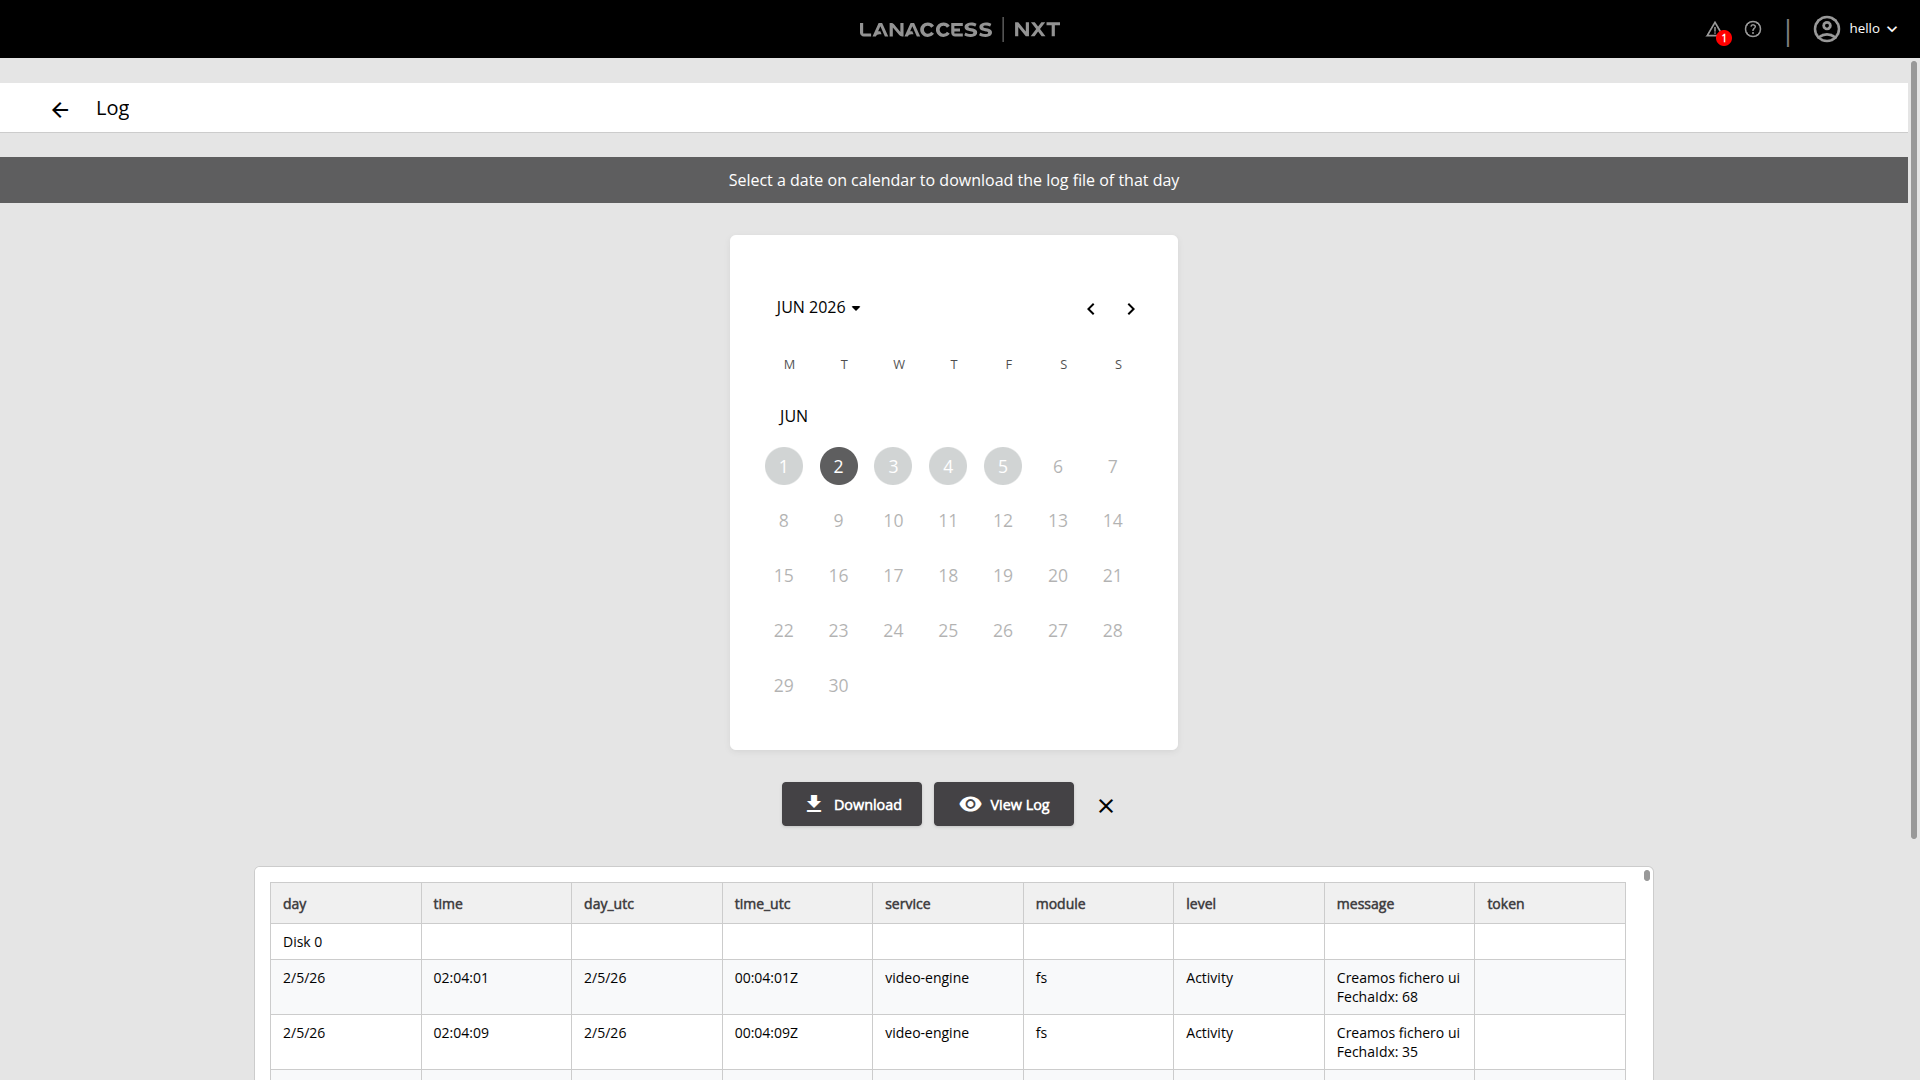
\includegraphics[width=0.95\textwidth]{figures/ui_log.png}
  \caption{Visor de registres i auditories amb filtres temporals i descàrrega.}
  \label{fig:ui_log}
\end{figure}

Per poder treballar amb volums de dades molt grans que poden superar les 500.000 files de successos per setmana, s'ha dissenyat un mètode de visualització optimitzat en dues capes que evita el col·lapse de la memòria RAM del navegador de l'usuari:
\begin{enumerate}
  \item \textbf{Sondeig de Calendari:} Abans de pintar la interfície del calendari, l'aplicació consulta a través de \texttt{commonCalendarGetDays.cgi} quins dies tenen fitxers de registre disponibles. El frontend marca exclusivament els dies actius al selector, evitant que l'operador hagi d'interrogar dates buides.
  \item \textbf{Processat de Dades amb SheetJS:} Quan es selecciona un dia vàlid, es demana l'historial a \texttt{listlog.cgi} com un fitxer binari xifrat estructurat. En lloc de renderitzar directament milers de línies al DOM (el que provocaria el bloqueig de la interfície de l'usuari), el frontend utilitza la llibreria \texttt{XLSX} (SheetJS) per parsejar les dades a nivell de memòria d'execució. El sistema organitza les dades en una taula reactiva de descàrrega i filtre local per paraula clau, permetent una navegació extremadament fluida.
\end{enumerate}

\subsection{Mòdul d'Ajuda i Documentació Integrada (Air-Gapped Operation)}
En entorns industrials o de màxima seguretat, és habitual que els gravadors NVR treballin en una xarxa aïllada físicament del món exterior (funcionament en entorns \textit{air-gapped}). En aquests casos, quan un tècnic necessita consultar una guia d'instruccions, no pot accedir a internet ni connectar-se a servidors corporatius de suport externs.

\begin{figure}[htbp]
  \centering
  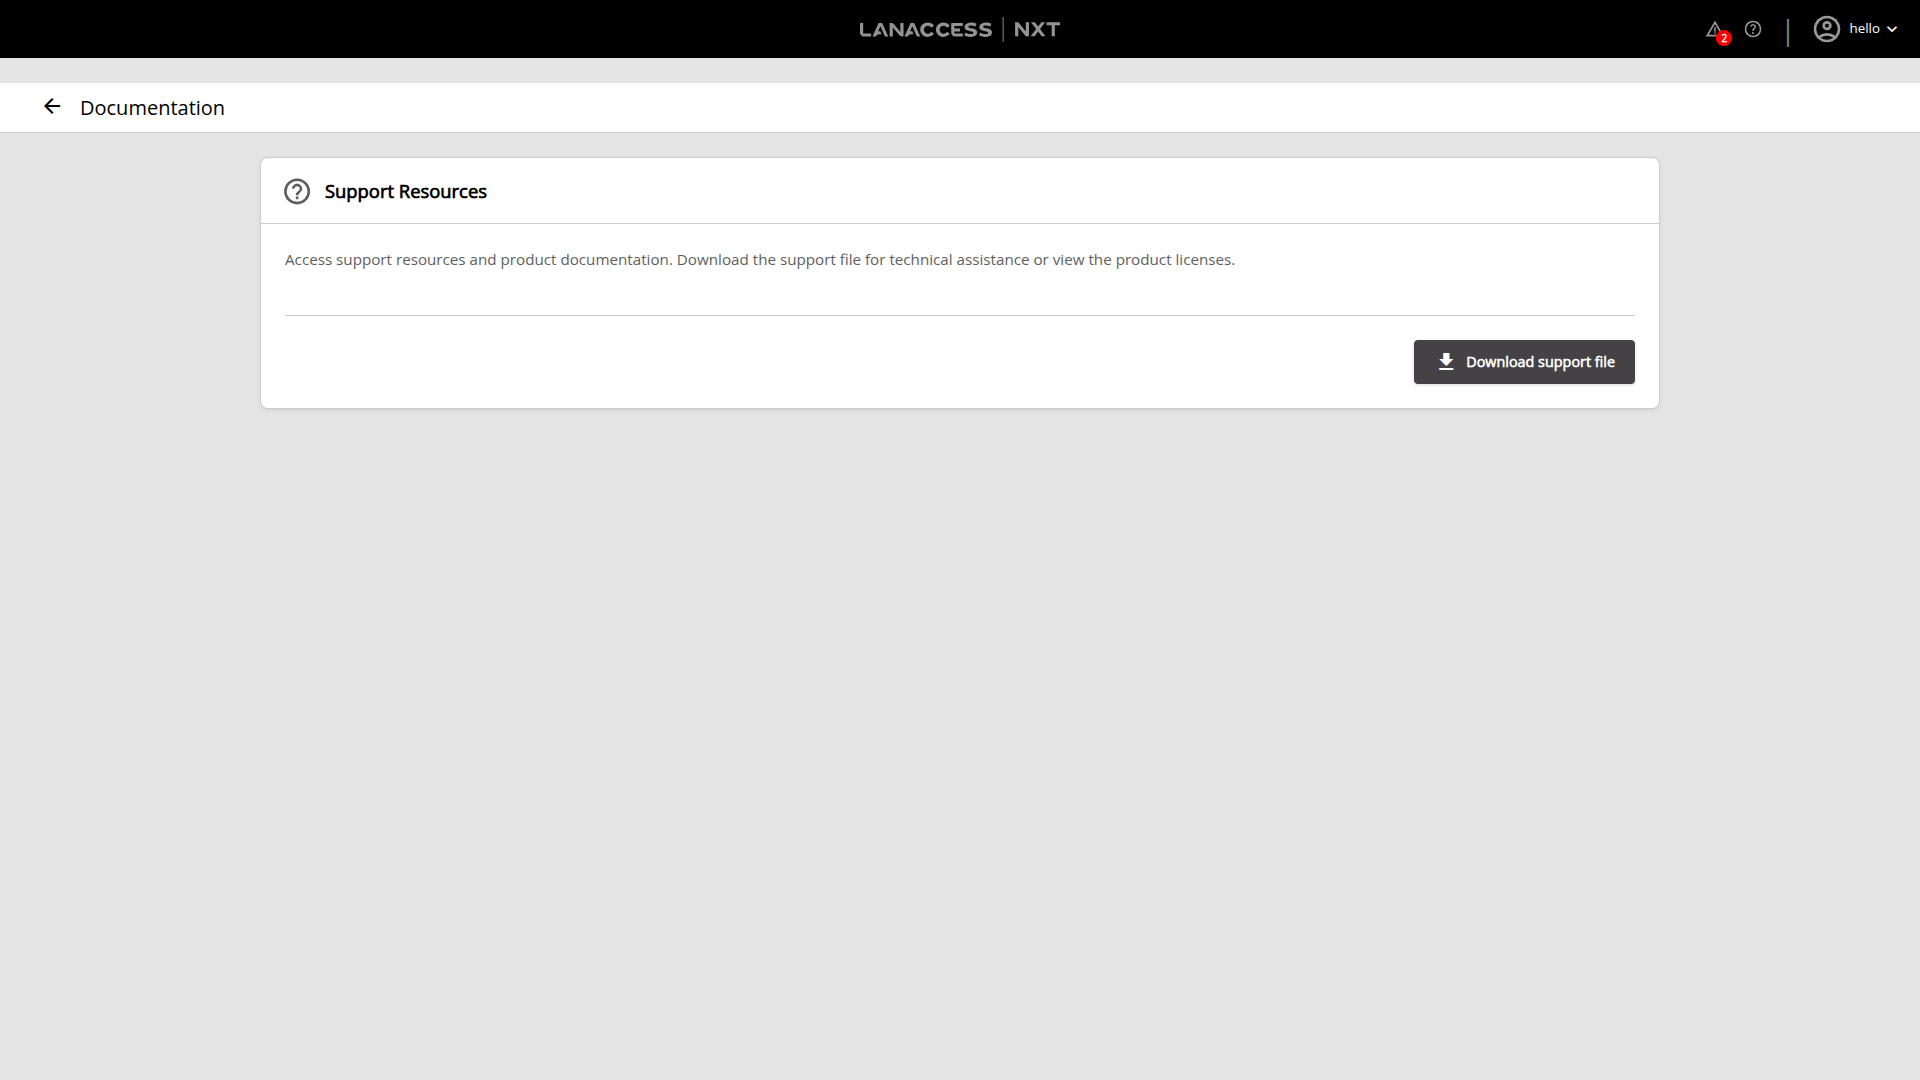
\includegraphics[width=0.95\textwidth]{figures/ui_documentation.png}
  \caption{Secció de suport tècnic per la descàrrega directa dels manuals en PDF.}
  \label{fig:ui_documentation}
\end{figure}

Per resoldre aquesta limitació operativa, la secció de Documentació (Figura \ref{fig:ui_documentation}) s'ha programat per funcionar de manera completament unificada i autosuficient. Tots els manuals d'usuari i fitxes tècniques estan integrats i empaquetats directament en la memòria de l'aplicació de l'equip. En fer clic sobre el botó de descàrrega del fitxer d'ajuda, el frontend envia una ordre cap al servei d'arxiu lògic de \texttt{la-core-legacy} per extreure el fitxer comprimit format \texttt{support\_file.tar.gz} del disc local i descarregar-lo al PC de l'instal·lador, oferint una eina d'ajuda autònoma i sense dependències de serveis externs de xarxa.

Garantint l'operativa completament desconnectada (\textit{air-gapped}) de la xarxa exterior de moltes d'aquestes màquines de seguretat, tota la documentació oficial d'ús i guies ràpides està introduïda en la mateixa memòria web del dispositiu (Figura \ref{fig:ui_documentation}). Mitjançant una vista senzilla que es comunica amb \textbf{la-core-legacy}, l'usuari només ha de clicar a la fila corresponent i l'arxiu PDF es descarregarà al seu PC sense requerir accés a portals web corporatius externs.